\documentclass[a4paper]{report}

%====================== PACKAGES ======================

\usepackage[french]{babel}
\usepackage[utf8x]{inputenc}
\usepackage{float}
\usepackage{amsmath}
\usepackage{xr}
\usepackage{graphicx}
\usepackage[colorinlistoftodos]{todonotes}
\usepackage{url}
\usepackage[colorlinks=true,urlcolor=blue]{hyperref}
\usepackage{array}
\usepackage{tabularx}
\usepackage{setspace}
\usepackage{abstract}
\usepackage[T1]{fontenc}
\usepackage[top=2cm, bottom=2cm, left=2cm, right=2cm]{geometry}
\usepackage{subfig}
\usepackage{multirow}
\usepackage{listings}
\usepackage{color}
\usepackage{hhline}
\definecolor{deepblue}{rgb}{0,0,0.5}
\definecolor{deepred}{rgb}{0.6,0,0}
\definecolor{deepgreen}{rgb}{0,0.5,0}
\usepackage{listings}
\usepackage{url}
\lstdefinestyle{numbers} {numbers=left, stepnumer=1, numberstyle=\tiny, numbersep=10pt}
\lstdefinestyle{MyFrame}{backgroundcolor=\color{white},frame=shadowbox}
\lstdefinestyle{MyBashStyle}{language=bash,style=numbers,style=MyFrame,frames=lines}
\lstdefinestyle{MyPythonStyle}{language=python,style=numbers,style=MyFrame,frame=lines}
\lstset{language=bash,frame=lines}
\lstset{language=python,frame=lines}

\newcommand\pythonstyle{\lstset{
language=Python,
style=numbers,
basicstyle=\ttfamily\scriptsize,
otherkeywords={self},{True},{False},             % Add keywords here
keywordstyle=\color{deepblue}\bfseries,
commentstyle=\color{deepred},
stringstyle=\color{deepgreen},
showstringspaces=false
frame=tb,
showstringspaces=false
}}

\newcommand\pythonexternal[2][]{{
\pythonstyle
\lstinputlisting[#1]{#2}}}


%====================== INFORMATION ET REGLES ======================

\setcounter{secnumdepth}{4}
\setcounter{tocdepth}{4}
\hypersetup{			
pdfauthor = {Florian GRANTE},	
pdftitle = {Monitoring : Mise en place d'une solution IoT avec Microsoft Azure},
pdfsubject = {Livrable 1},
pdfkeywords = {IoT, Microsoft, informatique, Azure, Raspberry pi},
pdfstartview={FitH}}
%======================== DEBUT DU DOCUMENT ========================
\begin{document}
\newcommand{\HRule}{\rule{\linewidth}{0.5mm}}
\begin{titlepage}
\begin{center}

% Upper part of the page. The '~' is needed because only works if a paragraph has started.

\includegraphics[width=0.8\textwidth]{./images/logo}~\\[1cm]

\textsc{\LARGE Stage : Service Aménagement Numérique}\\[1.5cm]

\textsc{\Large }\\[0.5cm]

% Title
\HRule \\[0.4cm]

{\huge \bfseries Dossier Bilan\\[0.4cm] }

\HRule \\[1.5cm]

% Author and supervisor
\begin{minipage}{0.4\textwidth}
\begin{flushleft} \large
\emph{Auteur:}\\
Florian \textsc{GRANTE}\\
\end{flushleft}
\end{minipage}
\begin{minipage}{0.4\textwidth}
\begin{flushright} \large
\emph{Superviseur:} \\
David \textsc{LAROSE}
\end{flushright}
\end{minipage}

\vfill

% Bottom of the page
{\large \today}

\end{center}
\end{titlepage}
\thispagestyle{empty}
\tableofcontents
\thispagestyle{empty}
\setcounter{page}{0}
\renewcommand{\arraystretch}{1.5}
%====================== INCLUSION DES PARTIES ======================
~
\thispagestyle{empty}
\setcounter{page}{0}
\newpage
\chapter*{Introduction}

\addcontentsline{toc}{chapter}{Introduction}


Au cours de mon mois de stage au service aménagement numérique de la ville de Drancy, j'avais pour objectif principal de réaliser une démonstration de faisabilité d'une station de monitoring pour bâtiments publiques. Tout était à faire, tant par le choix matériel que par la construction logiciel qui en découlait. J'ai également eu l'occasion de participer à un second projet dont je parlerais dans un second temps. Avant de délivrer mes conclusions sur ces projets, je tiens à remercier mon superviseur, M. LAROSE David pour sa confiance totale sur ce projet.
\chapter{Monitoring : Mise en place d’une solution IoT avec Azure}

Le but de ma mission était une la réalisation d'une démonstration de faisabilité d'une station permettant de relevé la température, l'humidité ou encore savoir si la lumière d'une pièce est allumée. Cette station a pour but d'être installée dans des bâtiments public comme des écoles par exemple. Le type de bâtiment n'est pas anodin puisqu'il ajoute des contraintes non négligeable pour l'installation des stations.

\section{Le cahier des charges}

Même si le nombre de contrainte est limité, elles conditionnent cependant le système à tel point qu'elle limite énormément les choix possibles :

\begin{enumerate}
\item Le système ne doit nécessité aucun pré-requis technique. J'ai réalisé un dossier d'installation du système que j'ai retenue pour cette mission. Ce dossier, devrait normalement remplir cette condition.
\item Le système ne doit communiquer uniquement par l'intermédiaire d'un câble Ethernet. Il n'est pas envisageable pour une mairie d'installer des systèmes sans fils dans une école primaire par exemple.
\item Pour offrir une liberté d'installation, la station doit s'affranchir d'une alimentation sur prise secteur.
\item les données doivent être consultable sur le \textit{Cloud Microsoft Azure}.
\item les données doivent en plus, être visible localement.
\end{enumerate}

Même si cela est succinct, je vais montrer au fur à mesure des choix que j'ai été amené à faire que ces conditions ont été déterminantes.

\section{La base de la station}
\subsection{La \textit{Raspberry Pi}}

\begin{figure}[H]
\begin{center}
		\makebox[\textwidth]{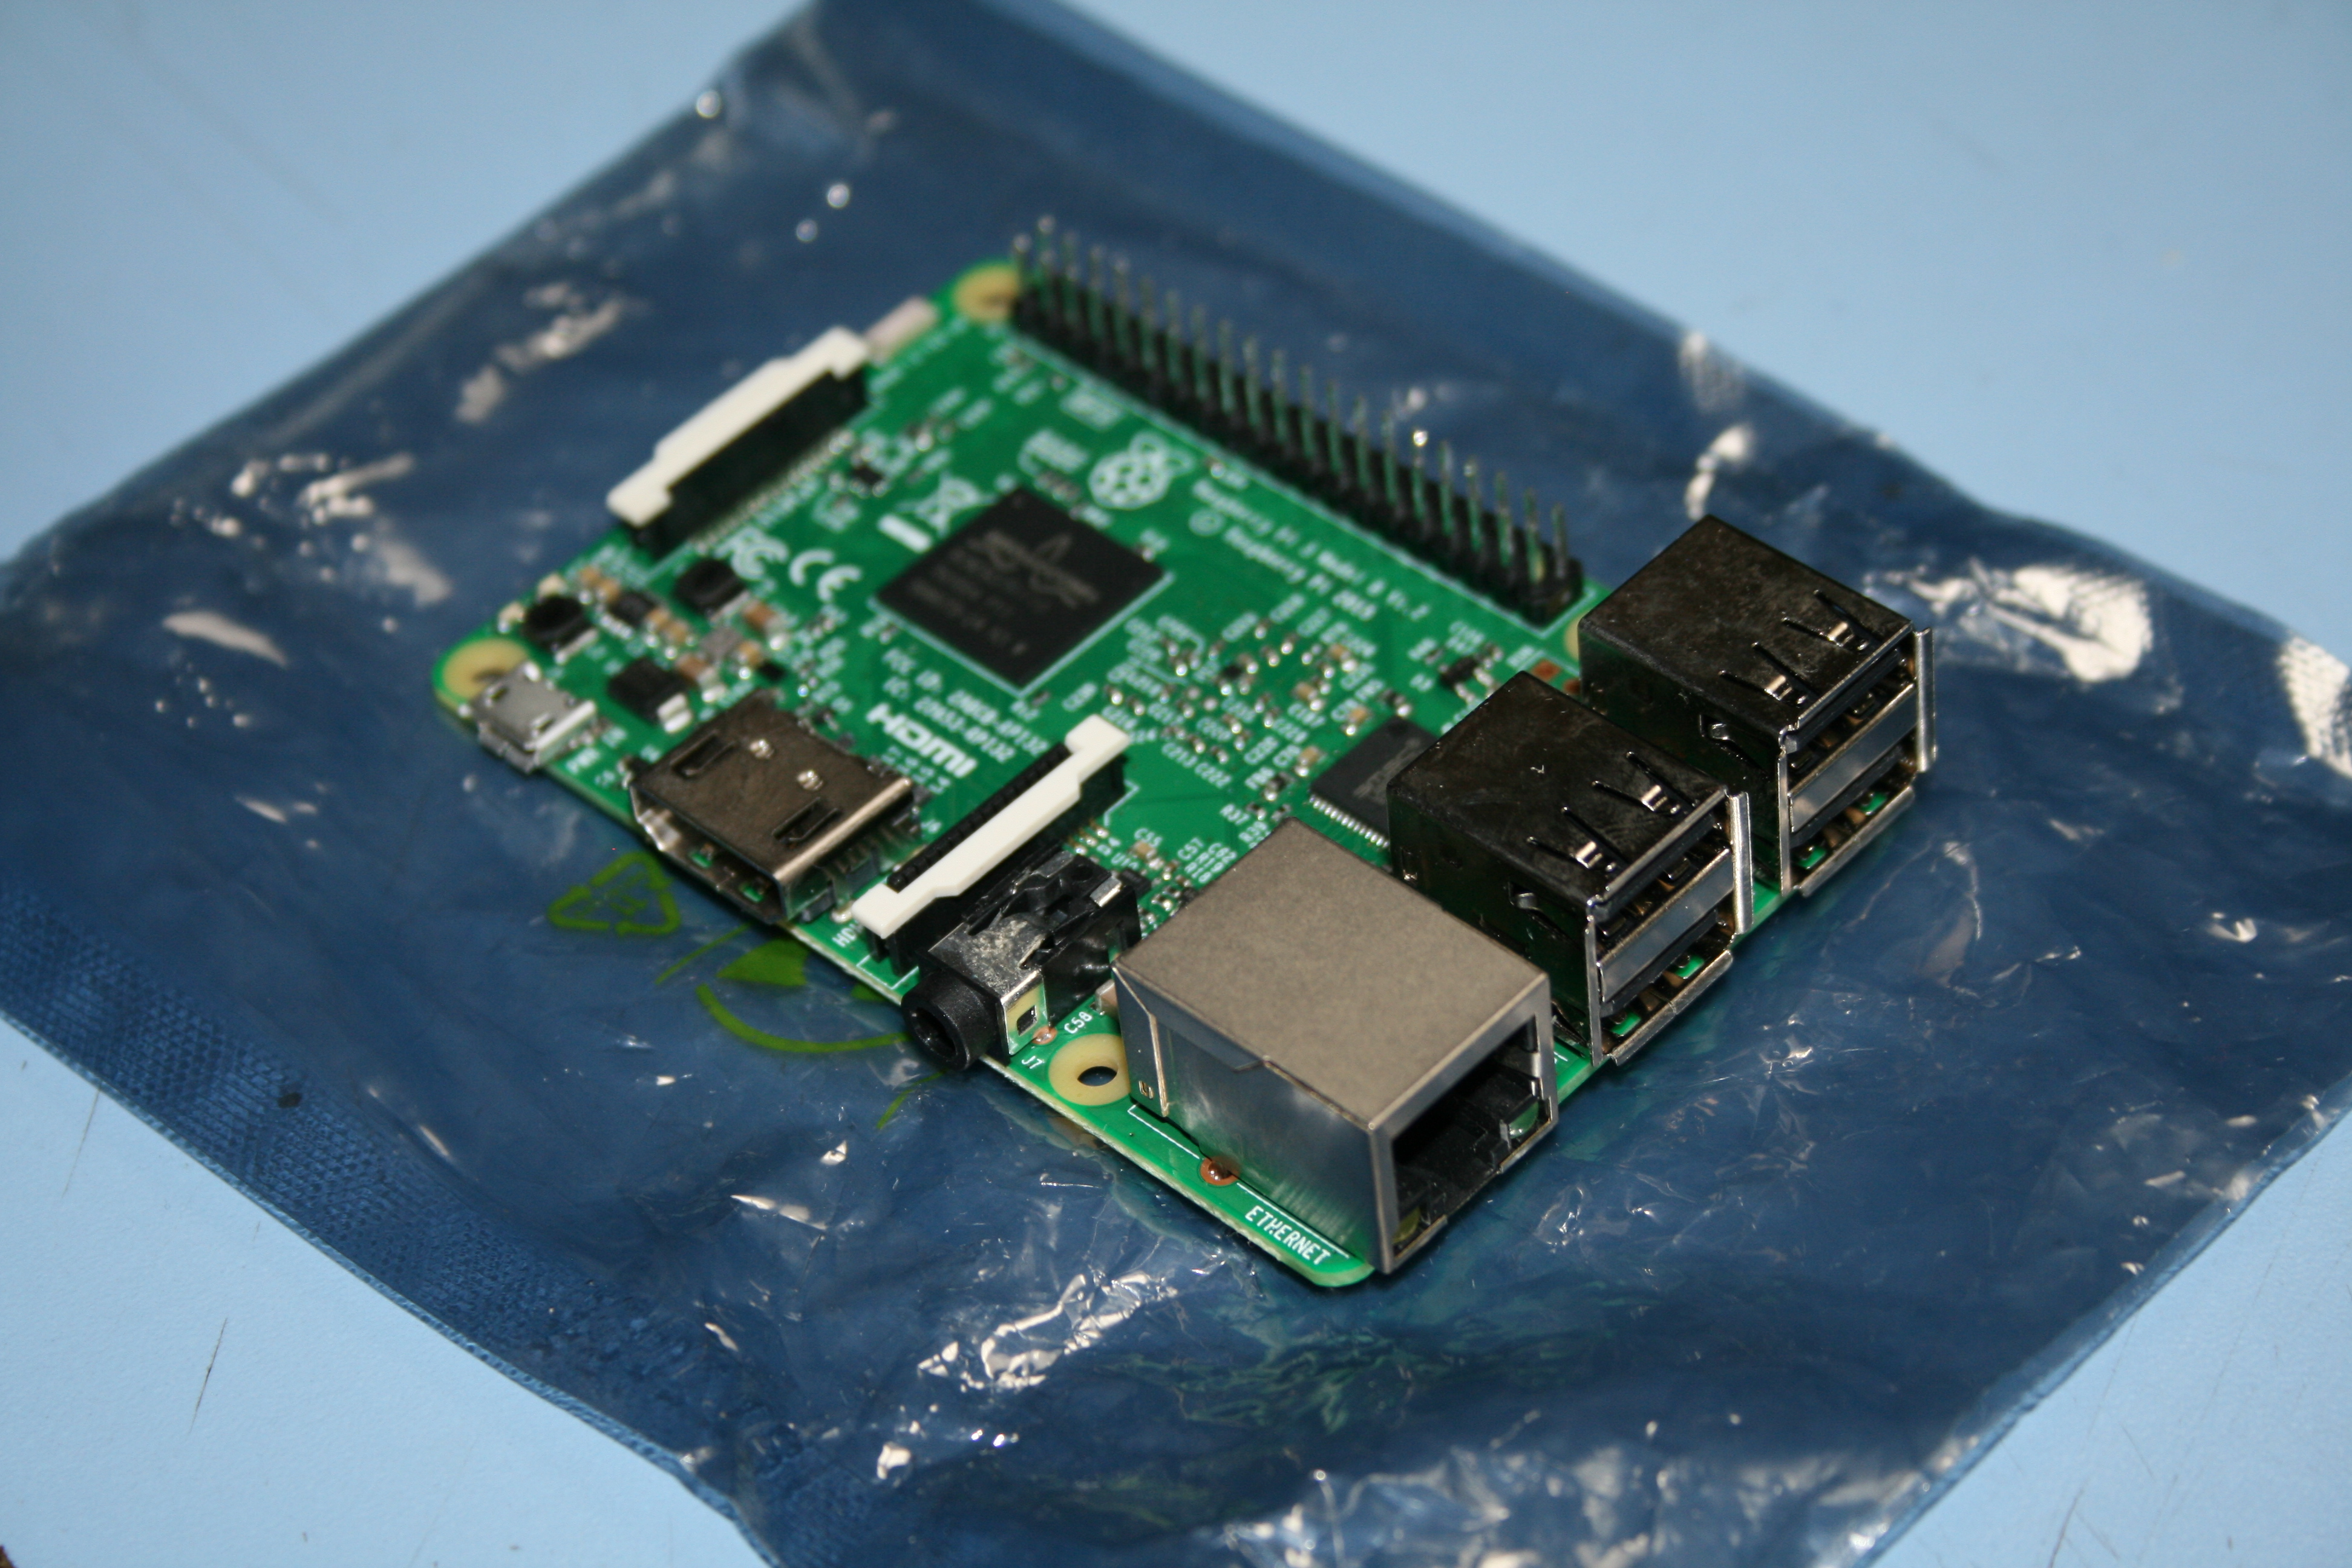
\includegraphics[width=.6\paperwidth]{images/rpi.jpg}}
\end{center}
		\caption{ \textit{Une Raspberry Pi}}
\end{figure}\\

La \textit{Raspberry Pi} est sans équivoque l'ordinateur du \textit{Maker} par excellence. Open source, elle permet de réaliser des systèmes embarqués performant pour un coût relativement faible et simple d'utilisation. Regardons ensemble les points du cahier des charges : 

\begin{enumerate}

\item Aucun pré-requis : Il s'agit ni plus ni moins que d'un ordinateur. J'ai détaillé cependant la façon dont on installe et configure l'OS pour la \textit{RaspberryPi}

\item Communication Ethernet : \textit{La Raspberry Pi}, comme tout bon ordinateur, possède une carte réseau et donc un port Ethernet. Noté toutefois, qu'à partir de la \textit{Raspberry Pi 3}, elle embarque également le \textit{Wi-Fi} et le \textit{Bluetooth}.

\item L'alimentation de la \textit{Raspberry Pi} se fait par un port micro-usb en \textit{5V}. La \textit{Raspberry Pi} ne gère pas l'alimentation \textit{PoE}. On peut alors recourir à une batterie ou bien à un \textit{PoE Splitter} qui récupère l'alimentation par le câble Ethernet et le transforme dans un port micro-usb.

\item Disposant d'une carte réseau, il n'y a aucun problème pour envoyer les données dans le cloud.

\item La \textit{Raspberry Pi} possède une sortie HDMI pour éventuellement brancher un écran. Il est également possible de mettre de petit écran LCD comme afficheur mais nous verrons ça plus tard.

\end{enumerate}

La \textit{Raspberry Pi} est alors un choix possible pour notre base de la station. Elle remplie effectivement toutes les conditions du cahier des charges.
\newpage
\subsection{\textit{L'Intel Edison}}

\textit{Intel} a décidé de se lancer dans l'IoT (il semblerait que le projet soit abandonnée) en sortant une puce : \textit{Edison}.
\begin{figure}[H]
\begin{center}
		\makebox[\textwidth]{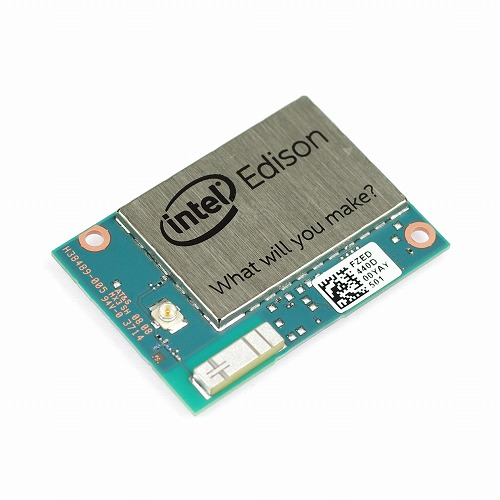
\includegraphics[width=.6\paperwidth]{images/edison.jpg}}
\end{center}
		\caption{ \textit{Une puce Edison}}
\end{figure}\\

Cette puce doit alors être placé sur une carte que fabrique également \textit{Intel} afin de pouvoir y brancher toute sorte de composants :\\

\begin{figure}[H]
\begin{center}
		\makebox[\textwidth]{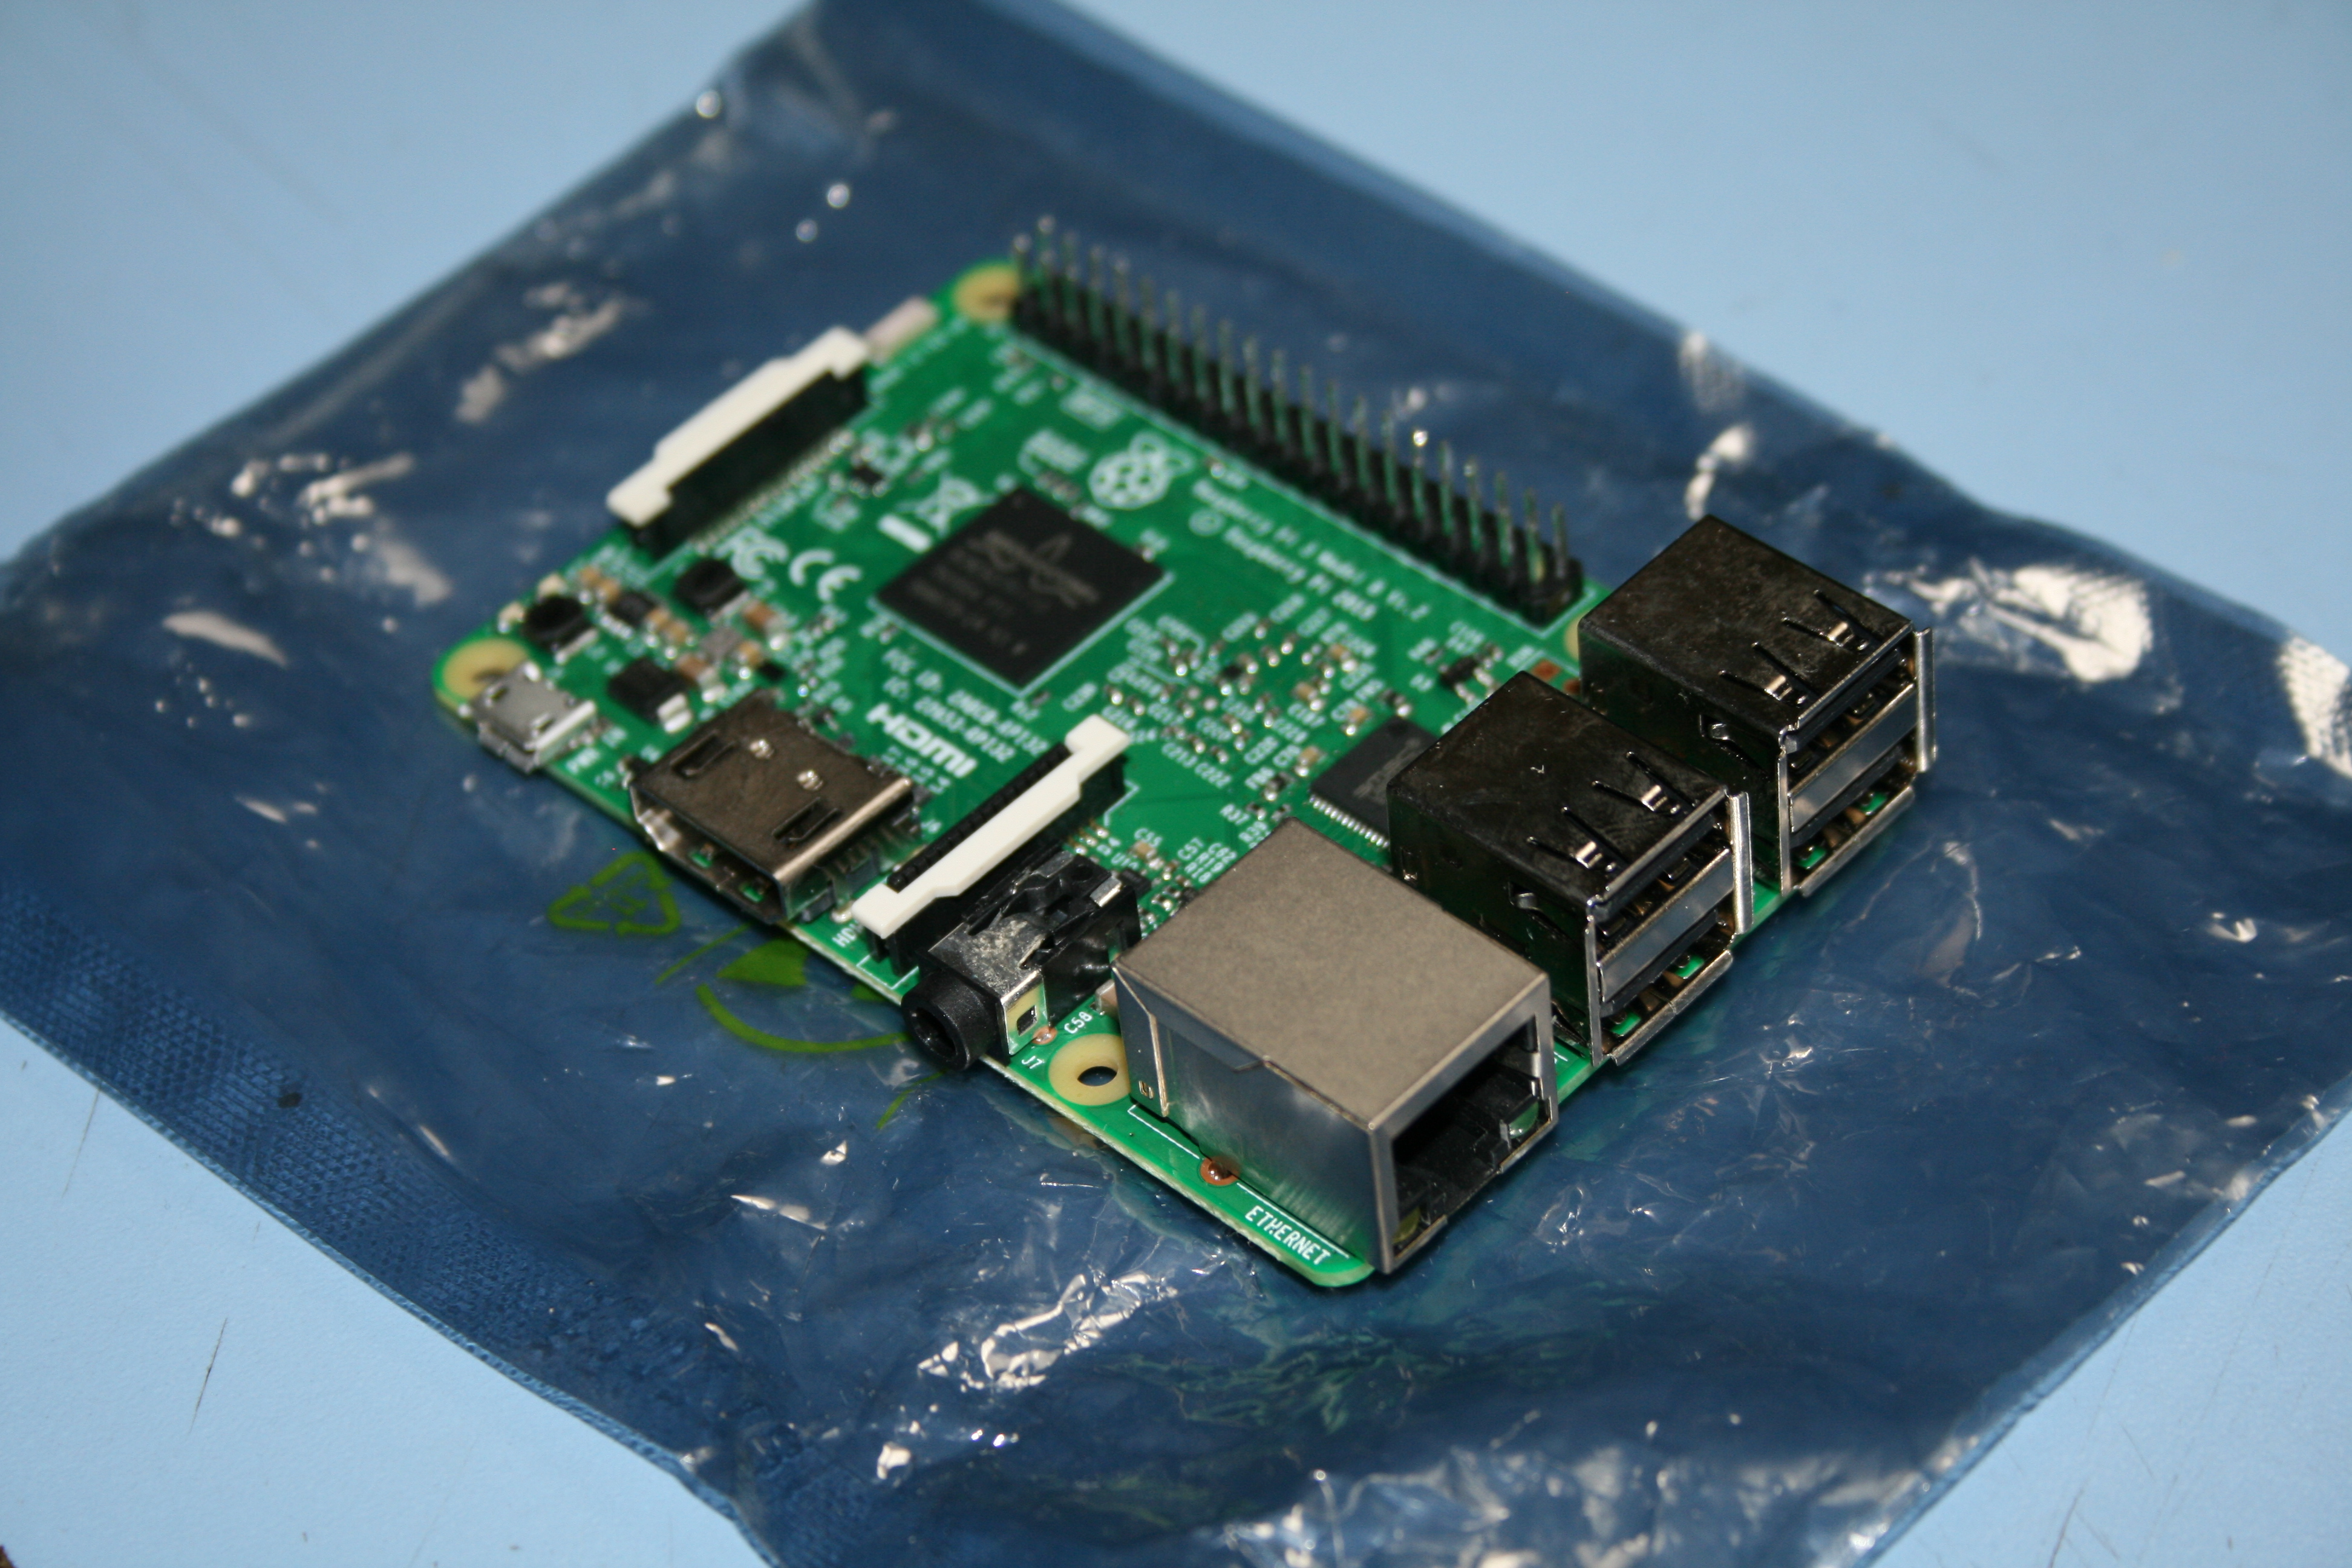
\includegraphics[width=.6\paperwidth]{images/rpi.jpg}}
\end{center}
		\caption{ \textit{Un intel Edison sur son board arduino}}
\end{figure}\\

Concrètement, il s'agit ni plus ni moins que d'un board Arduino amélioré. Amélioré par la performance de calcul de la puce \textit{Intel Edison} et amélioré car elle embarque un \textit{firmware} qui permet de compiler toute sorte de langage, dont le langage Arduino.\\

Le langage Arduino est parfait pour une mission comme la station car parfaitement adapté pour de l'électronique embarqué. Regardons les conditions du cahier des charges : 

\begin{enumerate}
\item Aucun pré-requis technique : De la même façon que pour la \textit{Raspberry Pi}, il suffit d'installer le \textit{firmware} dans une micro-SD par le biais d'un utilitaire très simple fournis par \textit{Intel}

\item L'intel ne dispose malheureusement pas ce carte réseau avec un port \textit{RJ45}. Il embarque cependant le \textit{Wi-Fi}. Comme ce dernier est embarqué sur un shield Arduino, on peut supposer qu'il est possible d'y installer un shield qui apporterais la fonctionnalité à notre système. Cela rendrait le système bien plus volumineux et complexe.

\item Ne possédant pas de port \textit{RJ45}, nous pouvons oublier la technologie \textit{PoE} sans l'utilisation d'un \textit{PoE Splitter} comme pour la \textit{Raspberry Pi}. L'alimentation pouvant se faire sur un micro-usb,il faudra donc opter pour la même solution.

\item Ayant la possibilité d'avoir un accès internet, il n'y aura donc aucun problème pour envoyer les données sur le \textit{Cloud Azure}. Il existe d'ailleurs de la documentation sur le site de \textit{Azure} concernant l'usage de \textit{L'intel Edison}.
\end{enumerate}

\textit{L'intel Edison} est donc un second choix possible même s'il est plus compliqué à mettre en place car nécessite plus de pièces.

\subsection{Le choix de la base de la station}

Comme je l'ai dit plus tôt, les deux choix sont possible. Il va alors falloir trancher au niveau du coût d'une part, puis de la simplicité de mise en place. Comme \textit{L'intel Edison} nécessite l'ajout d'un Shield pour pouvoir espérer un accès internet par câble, mon choix s'est porté sur la \textit{Raspberry Pi}.\\

\textit{L'intel Edison} se montre très intéressant de par sa puissance de calcul et ses possibilités, cependant, son coût est élevée et sa puissance se montre inutile pour l'usage que nous allons en avoir pour la station. Comme l'utilisation aurait été le même qu'un simple arduino uno, nous aurions pu envisager l'utilisation de ce dernier car il est un très bon choix en rapport qualité/prix. Il ne rivalise cependant pas en coût avec la \textit{Raspberry Pi}dès lors que nous ajoutons le shield Ethernet.\\

Ainsi, j'ai tout naturellement choisis la \textit{Raspberry Pi} pour réaliser la station. Il faut ensuite choisir les capteurs et autres composants que nous allons brancher à la \textit{Raspberry Pi}.

\section{Les composants}

Il faut maintenant faire une sélection de composants qui vont nous permettre de récolter les données, les afficher puis les envoyer dans le Cloud. Même si mon âme de roboticien voudrait créer une carte électronique où il suffirait de souder quelques composants pour avoir une plate forme faite sur mesure, il ne faut pas perdre de vu notre conditions "Aucun pré-requis". C'est pourquoi j'ai choisis d'utiliser les composants suivants : 

\subsection{Le Shield}

Pour réaliser une interface simpliste avec la \textit{Raspberry Pi} et les capteurs, nous allons utiliser un shield. Ce dernier porte le nom de \textit{GrovePi +}. 

\begin{figure}[H]
\begin{center}
	\makebox[\textwidth]{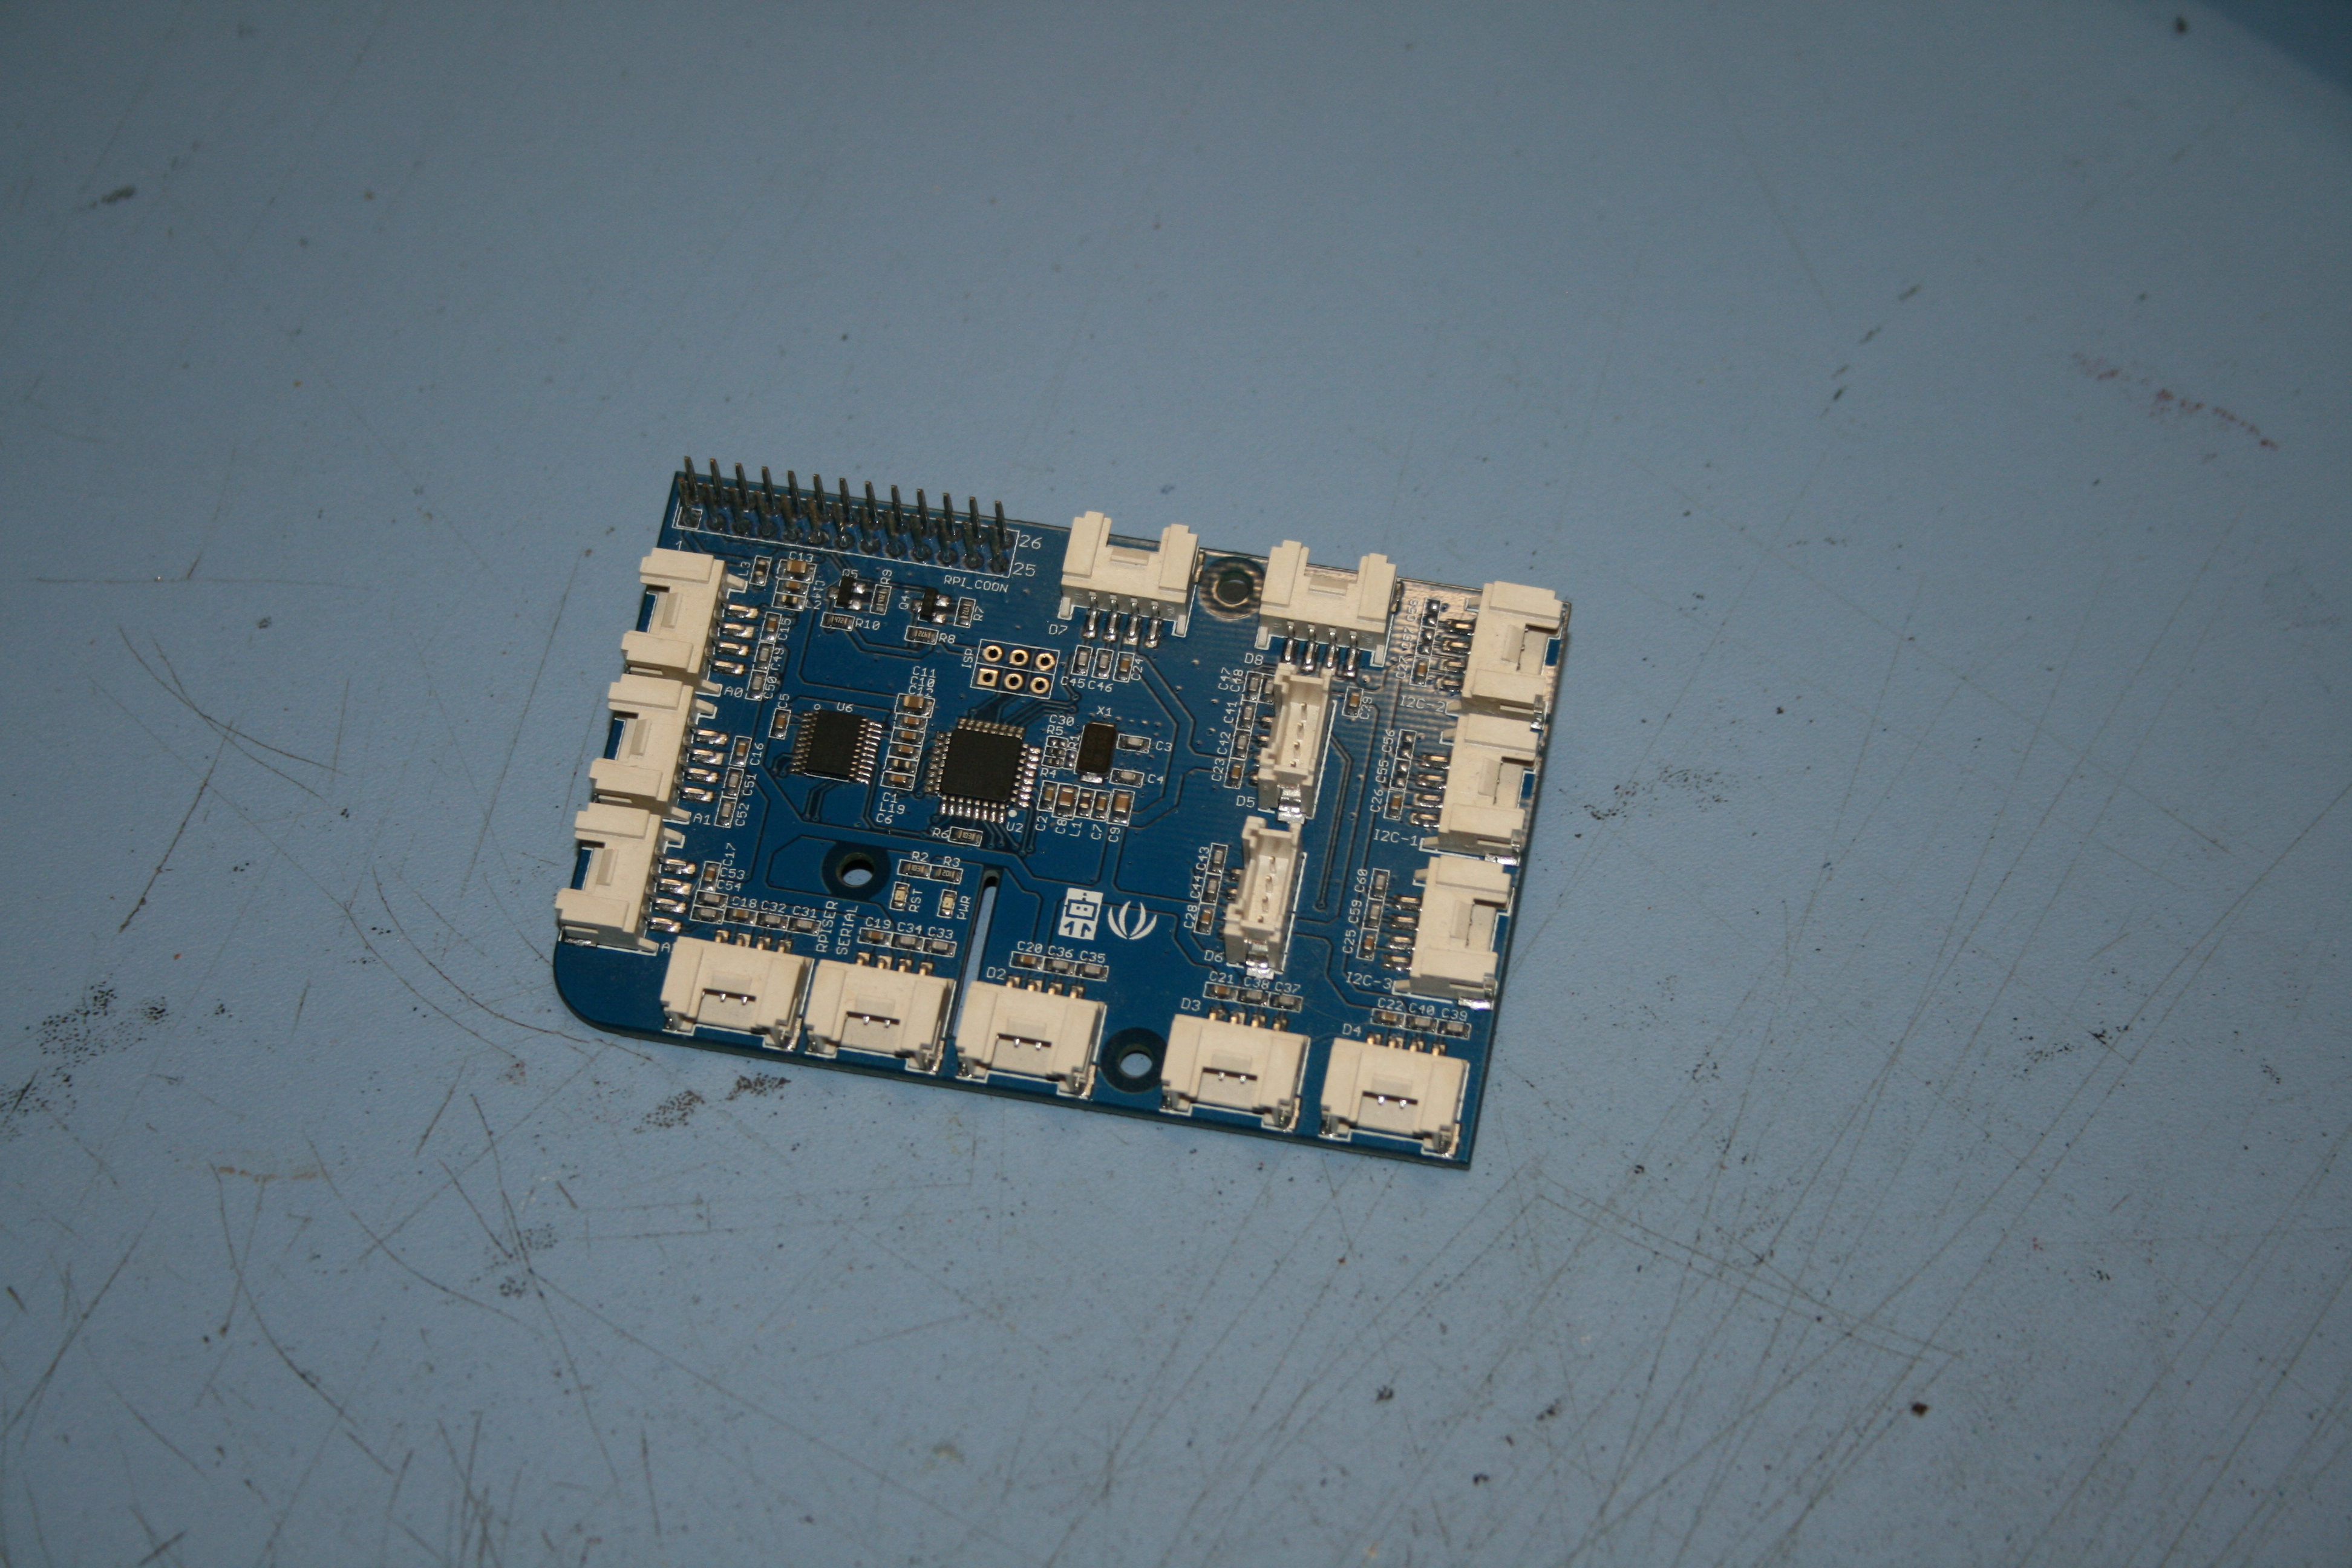
\includegraphics[width=.7\paperwidth]{images/grovepi.jpg}}
\end{center}
	\caption{ \textit{le Shield GrovePi+}}
\end{figure}\\

Pour \textit{l'Intel Edison} je parlais qu'il embarquait un board Arduino et compilais le langage Arduino (qui est ni plus ni moins qu'une version adapté de C++). Et bien ce shield est en réalité un Arduino qui communique avec la \textit{Raspberry Pi}. On notera le gros travail des ingénieurs qui ont réalisé les bibliothèques de tel sorte qu'il soit très facile de programmer pour l'utiliser mais nous détaillerons le langage de programmation dans une prochaine partie. Le seul bémol de ce Shield, c'est ses connecteurs 4-pin par lequel on branche les composants.\\

En effet, même s'il est simple et ludique de faire les branchements, cela oblige à acheter les composants qui sont déjà fabriqué pour être branché dessus. Du moins si l'on veut pas faire de soudure. Il serait possible de commander uniquement les connecteurs pour utiliser les composants que l'on souhaite mais ce n'est pas l'objectif ici.\\

\subsection{Capteur de température et d'humidité}

Le capteur que j'ai choisi ici est le DHT22.\\

Après plusieurs test avec son petit frère, le DHT11, j'ai décidé qu'il serait plus judicieux de monter en gamme car ce dernier manquait cruellement de précision. Ce genre de capteur sont cependant pas fait pour avoir une température instantanée. En effet, leur conception font qu'ils sont relativement lent pour réagir aux choc de température. Ces capteurs sont en effet là pour avoir une courbe de tendance de la température. Nous allons avoir l'allure de la variation de la température sur de longue durée de l'ordre de plusieurs heure. C'est pour ça qu'il n'est pas impossible de voir quelques valeurs faussée à quelques instants.\\

\subsection{Capteur de luminosité}

Les capteurs de luminosité sont très imprécis car la mesure de la luminosité avec précision coûte très chère. Cependant, nous n'avons pas besoin de mesurer de façon exacte la luminosité. D'une part car son unité, le luxmètre n'est pas très parlant pour le grand public et d'autre part, nous voulons juste avoir une information nous permettant de définir si la lumière d'une pièce serait allumée ou éteinte.\\

J'ai donc testé le capteur en le laissant tourner durant 2 jours complets pour voir un seuil à partir duquel on pouvait définir que la lumière était effectivement éteinte.\\

A noter cependant que ce seuil a été choisi arbitrairement et qu'il pourrait ne pas fonctionner selon les endroit où est placé la station (au bord d'une fenêtre typiquement).\\


\subsection{L'écran d'affichage}

Comme je l'ai spécifié dans le cahier des charges, il fallait pouvoir récupérer les valeurs localement. J'ai donc installé un écran afficheur 2x16 caractères.
De cette façon, la station pourra afficher les valeurs.\\

\subsection{L'encodeur rotatif}

L'écran ayant une capacité d'affichage limitée, j'ai ajouté un encodeur rotatif pour naviguer entre différents menu sur l'écran pour afficher différentes valeurs utile.\\

\subsection{PoE Splitter}

Le PoE Splitter va permettre d'alimenter la \textit{RaspberryPi} en PoE en découpant le câble RJ45 en 2 canaux : Un sur un câble micro - USB pour l'alimentation et un câble Ethernet RJ45 pour relier la station au réseau.

\section{Le langage de programmation}

Avec le \textit{Shield}, il était possible d'utiliser une multitude de langage de programmation. Cependant il fallait un langage intuitif et simple car il y a des lignes qui devront être changé lors d'un déploiement comme le nom des ressources sur Microsoft Azure où envoyer les données. J'ai automatiquement pensé au langage Python. Il est le langage de haut niveau par excellence. De plus, il est relativement adapté pour des script embarqué. Il n'est pas rare de voir des code de pilotage de robot fait en Python.

Voici un petit aperçu du code : 

\newpage
\pythonexternal{./station.py}\\

\section{Le coût d'une station}

Regroupons dans un premier temps le coût matériel, puis nous discuterons ensuite du coût logiciel, notamment sur \textit{Azure}.\\

\subsection{Coût du matériel}

Je vous propose donc le tableau ci-dessous réalisant l'inventaire des pièces nécessaire ainsi que de leur coût moyen en me basant sur deux sites : \textit{Amazon} et \textit{Seeed Studio}, qui est le distributeur de GrovePi+. Attention par contre à vérifier les provenance de Seeed car je me demande s'il n'est pas possible que des frais de douanes s'appliquent sur leur produits.

\begin{center}

	\begin{tabular}{|l|l|l|l|}
		\hline
		Composant & Prix & Amazon & Seeed \tabularnewline
		\hline
		RaspberryPi 3 & 35 euros & \href{ https://www.amazon.fr/Raspberry-Pi-Carte-M%C3%A8re-Model/dp/B01CD5VC92/ref=sr_1_3?s=computers&ie=UTF8&qid=1501236508&sr=1-3&keywords=raspberry+pi+3}{Amazon} & \href{https://www.seeedstudio.com/Raspberry%20Pi%203%20Model%20B-p-2625.html}{Seeed}\tabularnewline
		\hline
		Shield GrovePi+ & 33 euros & \href{https://www.amazon.fr/SEEEDSTUDIO-Seeedstudio-grovepi/dp/B01AFKN2TK/ref=sr_1_1?ie=UTF8&qid=1501238966&sr=8-1&keywords=grovepi%2B}{Amazon} & \href{https://www.seeedstudio.com/GrovePi%2B-p-2241.html}{Seeed}\tabularnewline
		\hline
		DHT22 & 17 euros & \href{https://www.amazon.fr/Accuracy-Temperature-Humidity-Raspberry-Platforms/dp/B01FY5EBO6/ref=sr_1_cc_1?s=aps&ie=UTF8&qid=1501239845&sr=1-1-catcorr&keywords=Temperature%26Humidity+Sensor+Pro}{Amazon} & \href{https://www.seeedstudio.com/Grove-Temperature%26Humidity-Sensor-Pro-p-838.html}{Seeed}\tabularnewline
		\hline
		Luminosite & 3 euros & & \href{https://www.seeedstudio.com/Grove-Light-Sensor-p-746.html}{Seeed}\tabularnewline
		\hline
		Ecran & 16 euros & \href{https://www.amazon.fr/gp/offer-listing/B01AFKPJ6O/ref=dp_olp_0?ie=UTF8&condition=all&qid=1501240259&sr=8-1}{Amazon} & \href{https://www.seeedstudio.com/Grove-LCD-RGB-Backlight-p-1643.html}{Seeed}\tabularnewline
		\hline
		Bouton rotatif & 5 euros & \href{https://www.amazon.fr/Seeedstudio-Grove-Capteur-Rotary-Angle-P/dp/B01AFKNFJM/ref=sr_1_fkmr0_3?ie=UTF8&qid=1501240488&sr=8-3-fkmr0&keywords=Grove+-+Rotary+Angle+Sensor%28P%29}{Amazon} & \href{https://www.seeedstudio.com/Grove-Rotary-Angle-Sensor%28P%29-p-1242.html}{Seeed}\tabularnewline
		\hline
		PoE Spliter & 10 euros & \href{https://www.amazon.fr/DSLRKIT-Active-Splitter-Ethernet-Raspberry/dp/B01H37XQP8/ref=sr_1_2?s=computers&ie=UTF8&qid=1501240606&sr=1-2&keywords=poe+splitter}{Amazon} &\tabularnewline
		\hline
		Micro SG (8Gb min) & 8 euros & & \tabularnewline
		\hline
		Total & 127 euros & &\tabularnewline
		\hline
	\end{tabular}
\end{center}\\

Nous avons donc un coût total moyen de l'ordre de 130€ par station. A noter qu'il s'agit d'un prix à l'unité, les commandes en gros jouissant de réduction sur Seeed Studio.\\

De plus, compter 2 à 3 euros de matière plastique si vous voulez imprimer un bouton et une coque (on ne rentrera pas l'imprimante 3D dans le coût).\\

\subsection{Coût logiciel}

Côté logiciel, j'ai utilisé un OS \textit{OpenSource} et crée le code pour le bon fonctionnement de la station. Les logiciels tiers pour la configuration sont entièrement gratuit.\\

Le seul coût vient alors sur le Cloud \textit{Azure}.\\

Mes estimations sont à revoir avec un conseiller chez \textit{Microsoft Azure} car je ne suis pas certain.\\

J'estime le tarif à minimum 1







\chapter{Configuration de la station}

\section{Création et installation de la distribution \textit{Raspbian}.}

Pour une \textit{RaspberryPi}, son disque dur est nul autre qu'une carte Micro SD. C'est donc sur ce support que vous allez faire l'installation.

Pour réaliser cette étape, vous aurez besoin de :
\begin{itemize}
	\item d'une \textit{RaspberryPi}
	\item d'une carte micro SD de minimum 8Go
	\item du logiciel \href{etcher.io}{Etcher}
	\item de \href{https://sourceforge.net/projects/dexterindustriesraspbianflavor/}{\textit{Raspbian}}. En réalité il s'agit d'une version modifiée par la société Dexter Industries qui est spécialisé dans l'utilisation de \textit{RaspberryPi} pour la robotique.
	\item d'un adaptateur pour relier la micro SD à votre ordinateur.
\end{itemize}\\
Vous pouvez désormais commencer l'installation de l'OS sur notre \textit{RaspberryPi}

\begin{enumerate}
	\item Connecter la micro SD sur votre ordinateur.\\
	\item Lancer le logiciel \textit{Etcher}\\
	\begin{figure}[H]
	\begin{center}
		\makebox[\textwidth]{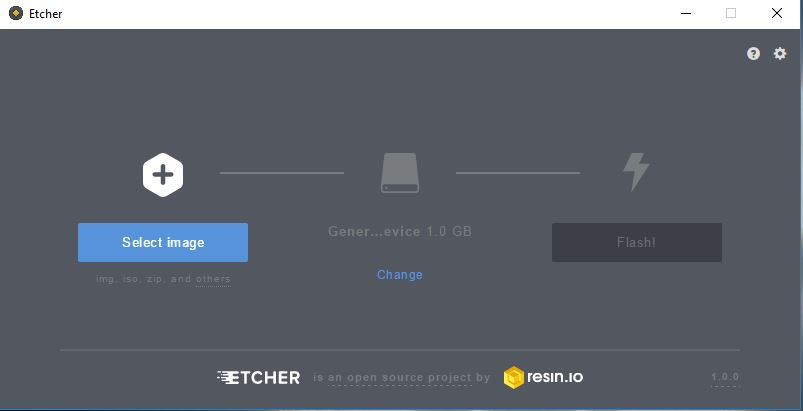
\includegraphics[width=.6\paperwidth]{images/etcher1.jpg}}
	\end{center}
		\caption{ \textit{Logiciel Etcher au lancement}}
	\end{figure}\\
	\item Cliquer sur \textit{"Select image"} à gauche puis sélectionner le fichier \textit{.zip} récupéré depuis le site \textit{SourceForce} dans les pré-requis.\\
	\item Vérifier que le périphérique qui est renseigné au centre est bien la micro SD. Dans le cas contraire cliquer sur \textit{"Change"}.\\
\newpage
	\item Si les deux étapes précédentes sont OK, cliquer sur \textit{"Flash"}.\\
	\begin{figure}[H]
	\begin{center}
		\makebox[\textwidth]{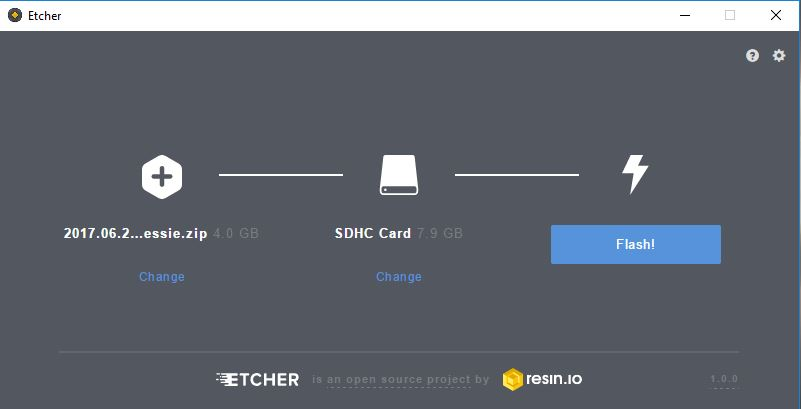
\includegraphics[width=.6\paperwidth]{images/etcher2.jpg}}
	\end{center}
		\caption{ \textit{Etcher prêt à flasher}}
	\end{figure}\\
\end{enumerate}
Et voilà, l'opération peut prendre une dizaine de minutes. C'était simple non ?

\section{Première mise en route de la \textit{RaspberryPi}.}

\begin{enumerate}

	\item Maintenant que vous avez \textit{Raspbian}, vous allez pouvoir démarrer votre nouvel ordinateur.
Pour cela, il vous suffit d'insérer la microSD au dos de la \textit{RaspberryPi}.\\
\begin{figure}[H]
\begin{center}
	\makebox[\textwidth]{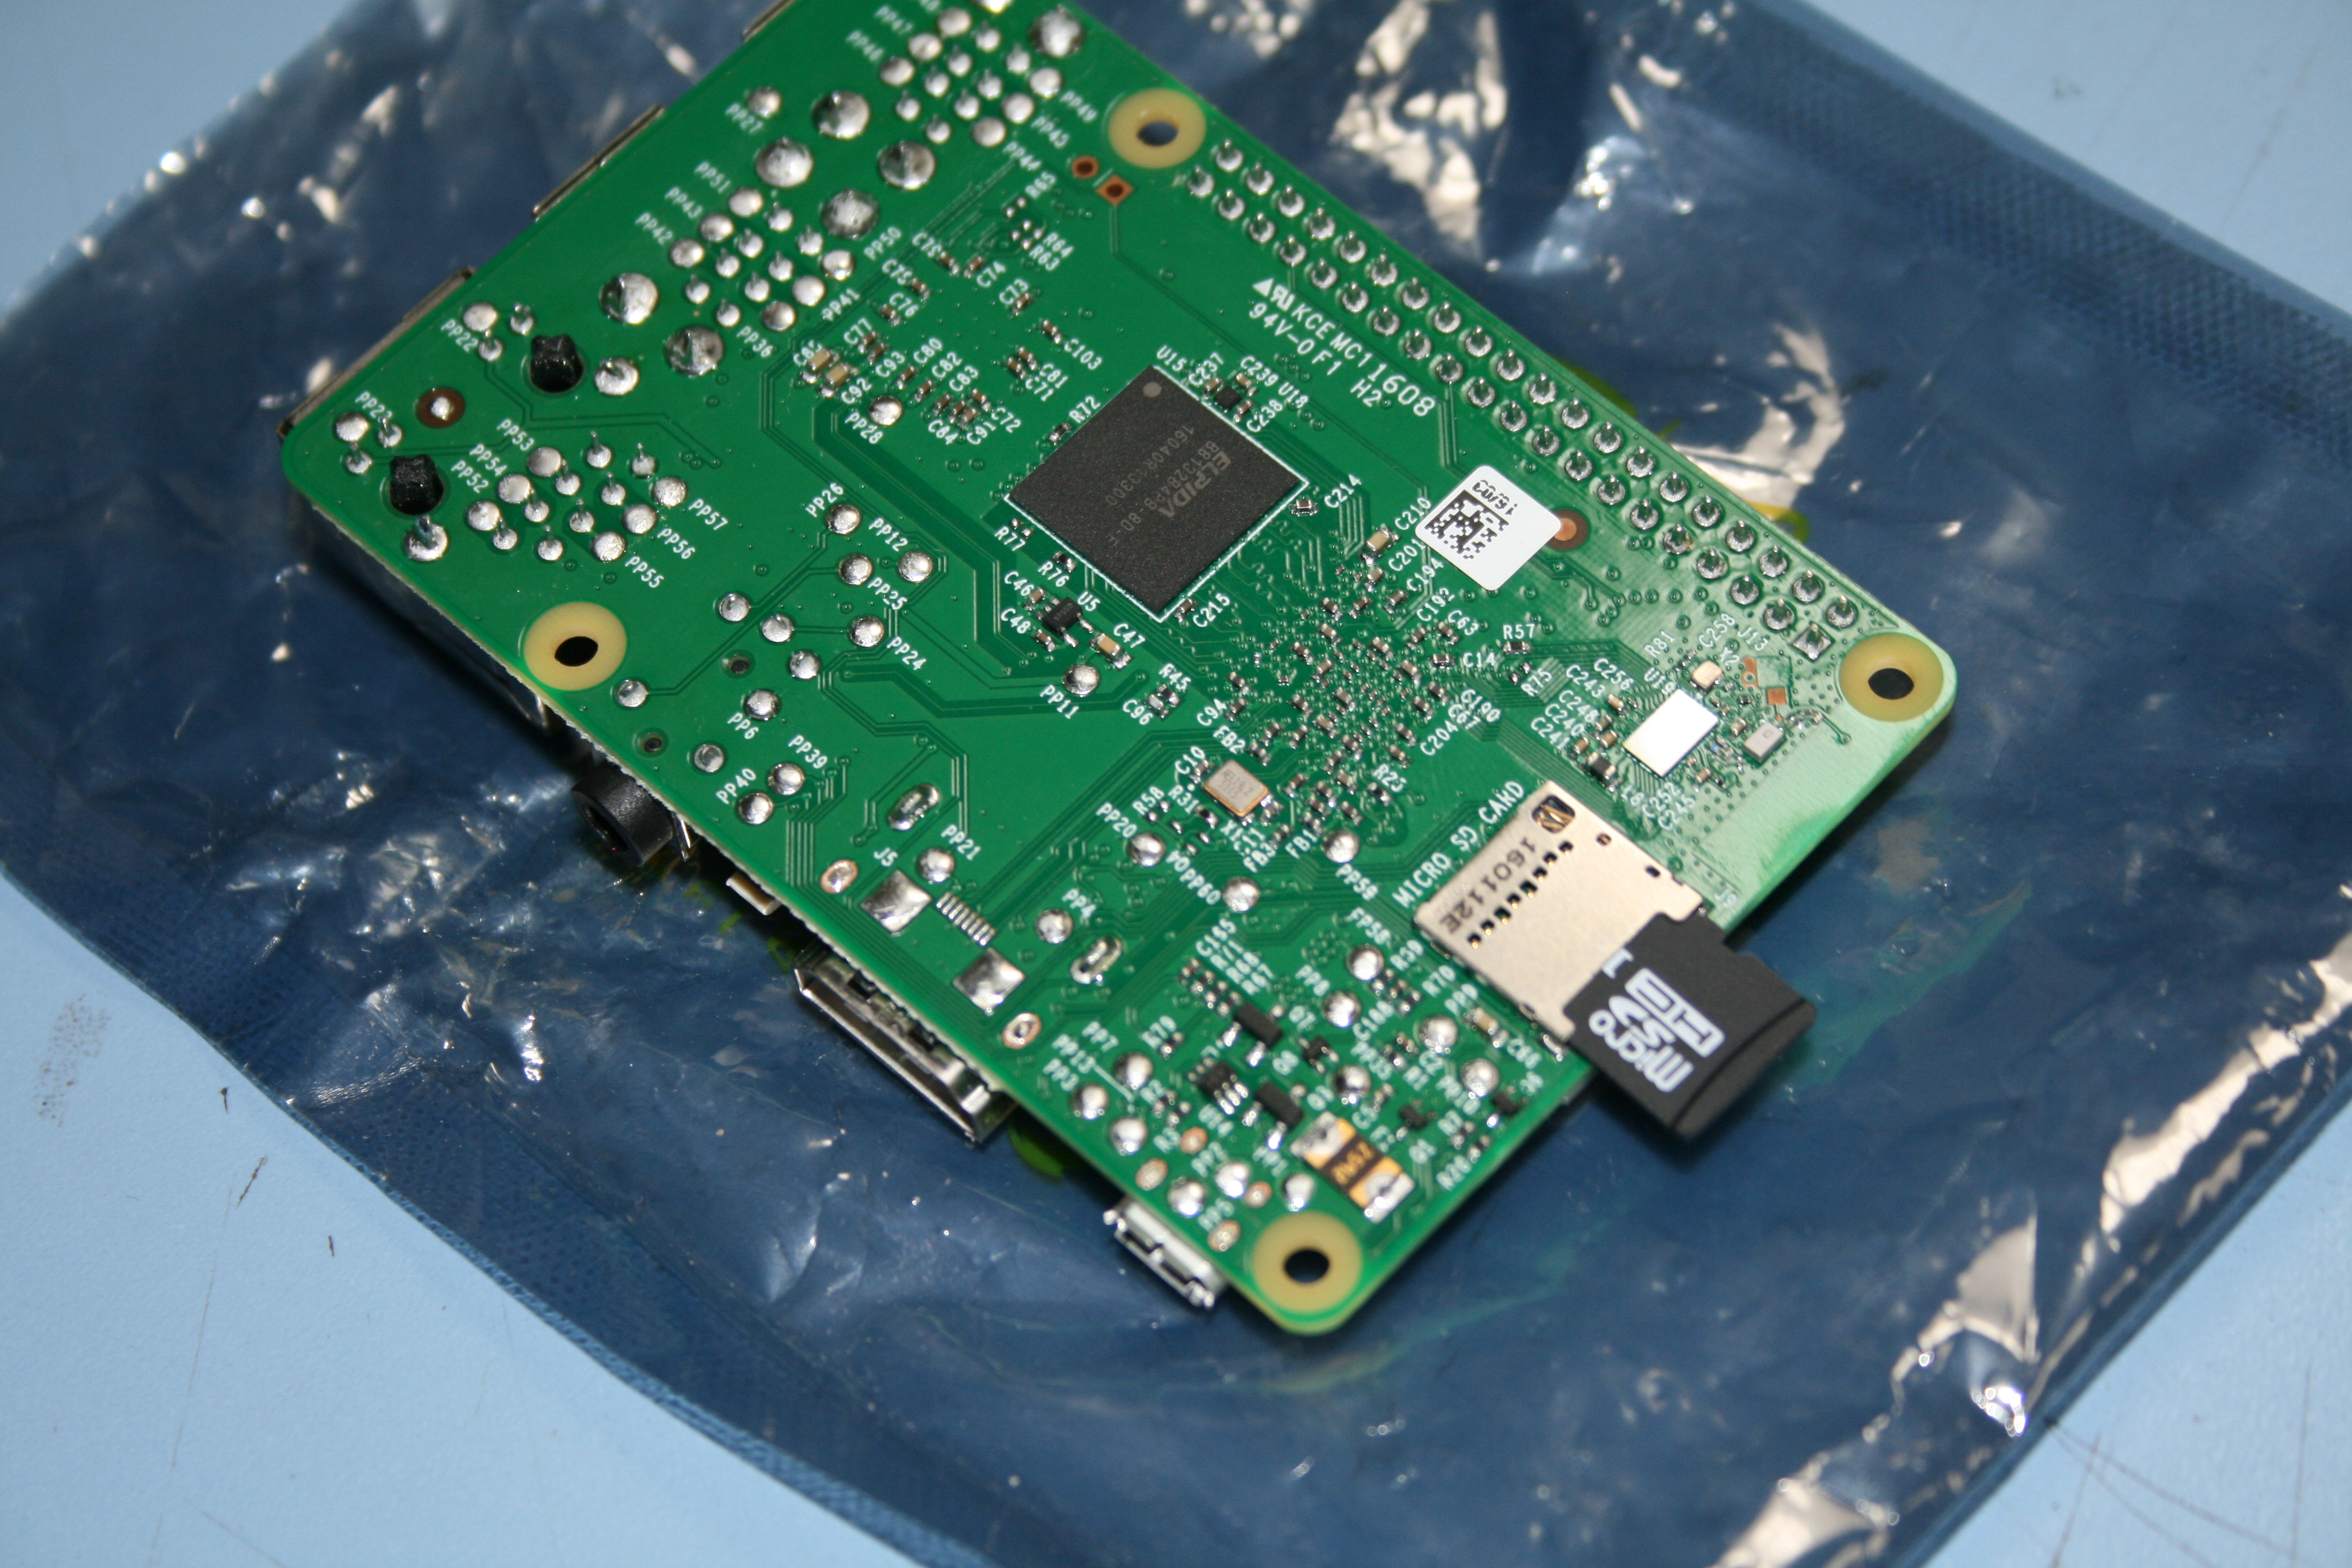
\includegraphics[width=.6\paperwidth]{images/microsd.jpg}}
\end{center}
	\caption{ \textit{La \textit{RaspberryPi} de dos}}
\end{figure}\\

	\item Avant de l'alimenter, nous allons distinguer deux cas.. Si vous avez la possibilité, de façon extérieur, d'accéder à l'adresse IP de votre \textit{RaspberryPi} alors vous pouvez sauter l'étape N°3. Si cela n'est pas possible, brancher un écran et un clavier & souris.\\
	Vous pouvez maintenant l'alimenter en utilisant le port micro USB qui est à côté du port HDMI.\\

\newpage
	
	\item Si vous suivez cette étape, vous devriez voir apparaître des lignes de commandes qui défilent. Quelques instants plus tard, vous arrivez sur l'environnement de bureau de votre \textit{RaspberryPi}. Sur ce bureau, ouvrez un terminal en cliquant sur l'écran en haut à gauche : 
	
\begin{figure}[H]
\begin{center}
	\makebox[\textwidth]{
\includegraphics[width=.6\paperwidth]{images/terminal.jpg}}
\end{center}
	\caption{ \textit{Barre de tâche de Raspbian}}
\end{figure}\\

Une fois le terminal ouvert, entrer la commande suivante :
\begin{lstlisting}[style=MyBashStyle]
	sudo ifconfig
\end{lstlisting}\\

un mot de passe devrait vous être demandé, par défaut, le mot de passe est "robots1234".
Vous devriez avoir un résultat de ce type :\\

\begin{figure}[H]
\begin{center}
	\makebox[\textwidth]{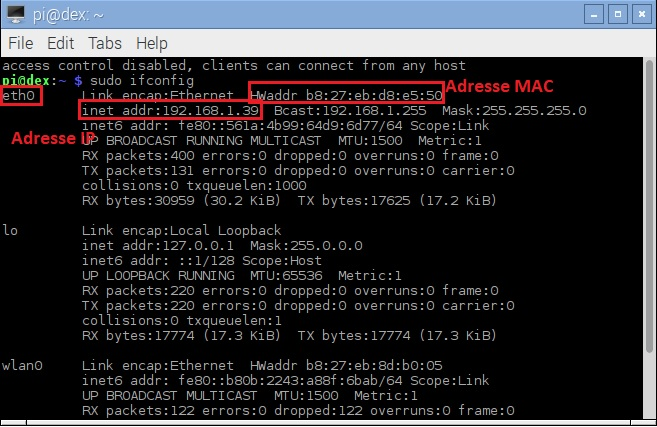
\includegraphics[width=.6\paperwidth]{images/ip_mac.jpg}}
\end{center}
	\caption{ \textit{Résultat de la commande sudo ifconfig}}
\end{figure}\\

Vous pouvez ainsi récupérer l'adresse IP et adresse MAC si nécessaire pour gérer votre réseau. Pour l'adresse IP, selon l'architecture de votre réseau, il s'agit d'une adresse privé ou public. Dans le premier cas, vous serez obligé d'être dans le même réseau pour y accéder, dans le second pas de problème quelque soit l'endroit où vous vous trouver.
Maintenant que vous avez récupérer l'adresse IP, vous pouvez débrancher tous les périphériques de votre \textit{RaspberryPi} et laisser uniquement l'alimentation et le câble ethernet.

	\item Très bien, désormais que vous avez l'adresse IP à disposition, vous pouvez installer le nécessaire pour utiliser nos capteurs. Vous pourriez très bien continuer cette installation directement sur la \textit{RaspberryPi} mais si vous n'avez jamais fait ce qui va suivre, cela vous fera un bon entrainement.\\

\begin{enumerate} 
	\item Télécharger et installer le logiciel \href{https://git-for-windows.github.io/}{Git Bash}. Ce logiciel permet l'utilisation d'un terminal plus avancé et compatible avec le langage système \textit{Bash}.
	\item Lancer \textit{Git Bash}
	\item taper la commande en remplaçant "xxx.xxx.xxx.xxx" par l'adresse IP de la \textit{RaspberryPi}\\
	\begin{lstlisting}[style=MyBashStyle]
	ssh pi@xxx.xxx.xxx.xxx
	\end{lstlisting}\\
la première fois, il vous sera demander si vous voulez réellement vous connecter sur le périphérique, taper alors "yes" puis sur la touche \textit{Entrée}
	\item Le mot de passe est "robots1234". Si tout c'est bien passé, vous devriez avoir cet aperçu :\\
	\begin{figure}[H]
	\begin{center}
		\makebox[\textwidth]{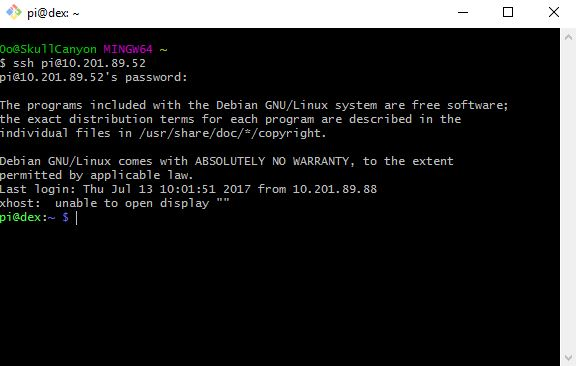
\includegraphics[width=.6\paperwidth]{images/ssh.jpg}}
	\end{center}
		\caption{ \textit{connexion à la RaspberryPi en SSH}}
	\end{figure}\\
	
	\item vous naviguez maintenant dans la \textit{RaspberryPi}. Dans un premier temps, il va falloir changer le mot de passe car celui ci est un mot de passe par défaut. Enter la commande :\\
	\begin{lstlisting}[style=MyBashStyle]
	sudo raspi-config
	\end{lstlisting}\\
	un menu sur fond bleu devrait apparaitre :\\
	
\begin{figure}[H]
\begin{center}
	\makebox[\textwidth]{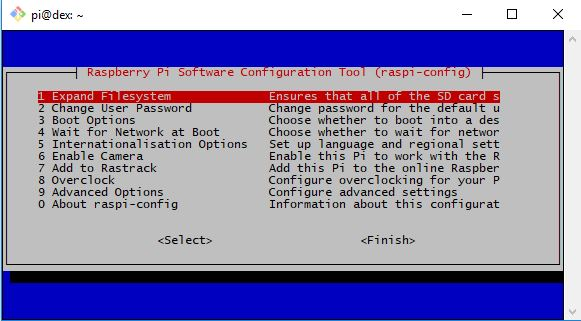
\includegraphics[width=.6\paperwidth]{images/raspiconfig.jpg}}
\end{center}
	\caption{ \textit{Menu Raspi-config}}
\end{figure}\\

Premièrement, choisissez la première option \textit{Expand Filesystem}. Cela va faire en sorte que \textit{Raspbian} occupe toute la micro SD. Une fois terminé, choisissez la seconde option. Nous allons changer le mot de passe par défaut "robots1234". Il va vous être demandé de saisir 2 fois un nouveau mot de passe. Pas de panique, lorsque l'on tape un mot de passe sous linux, aucun caractère apparait !
	
	\item Quitter le menu en choisissant l'option \textit{"Finish"}. Il vous sera demandé de redémarrer la \textit{RaspberryPi}. Après quelques temps, refaite l'étape \textit{c & d} mais avec le nouveau mot de passe qui a été renseigné.
	\item Maintenant, vous pouvez installer GrovePi pour pouvoir utiliser le \textit{Shield}. Entrer alors les deux commandes suivantes :\\
	\begin{lstlisting}[style=MyBashStyle]
	sudo curl https://raw.githubusercontent.com/DexterInd
	/Raspbian_For_Robots/master/upd_script/fetch_grovepi.sh | bash
	 
	sudo reboot
	\end{lstlisting}\\
	Votre \textit{RaspberryPi} va redémarrer.
	\item Connecter vous à nouveau en "ssh" comme pour l'étape 4 mais cette fois ci avec votre nouveau mot de passe.
	\item Réaliser alors cette suite de commande une à une. Appuyer sur la touche \textit{Entrée} lorsque l'on vous demande de continuer :
	\begin{lstlisting}[style=MyBashStyle]
	cd
	sudo git clone https://github.com/DexterInd/GrovePi
	cd GrovePi/Script
	sudo chmod +x install.sh
	sudo ./install.sh
	\end{lstlisting}\\
	
	\item Vous devriez à la fin obtenir un écran similaire à la photo précédente.\\ 
	Effectuer alors la commande :
	\begin{lstlisting}[style=MyBashStyle]
	sudo shutdown now
	\end{lstlisting}\\
	Elle va alors s'arrêter. Vous pouvez alors la débrancher après quelques instant.
	\end{enumerate}\\
	
		\item Vous pouvez désormais ajouter le \textit{Shield} sur la \textit{RaspberryPi} Comme ci-dessous \textbf{ATTENTION AU BROCHES UTILISÉES, BRANCHER LE SHIELD DANS LA MÊME CONFIGURATION QUE SUR LA PHOTO !}\\
		
	\begin{figure}[H]
	\begin{center}
		\makebox[\textwidth]{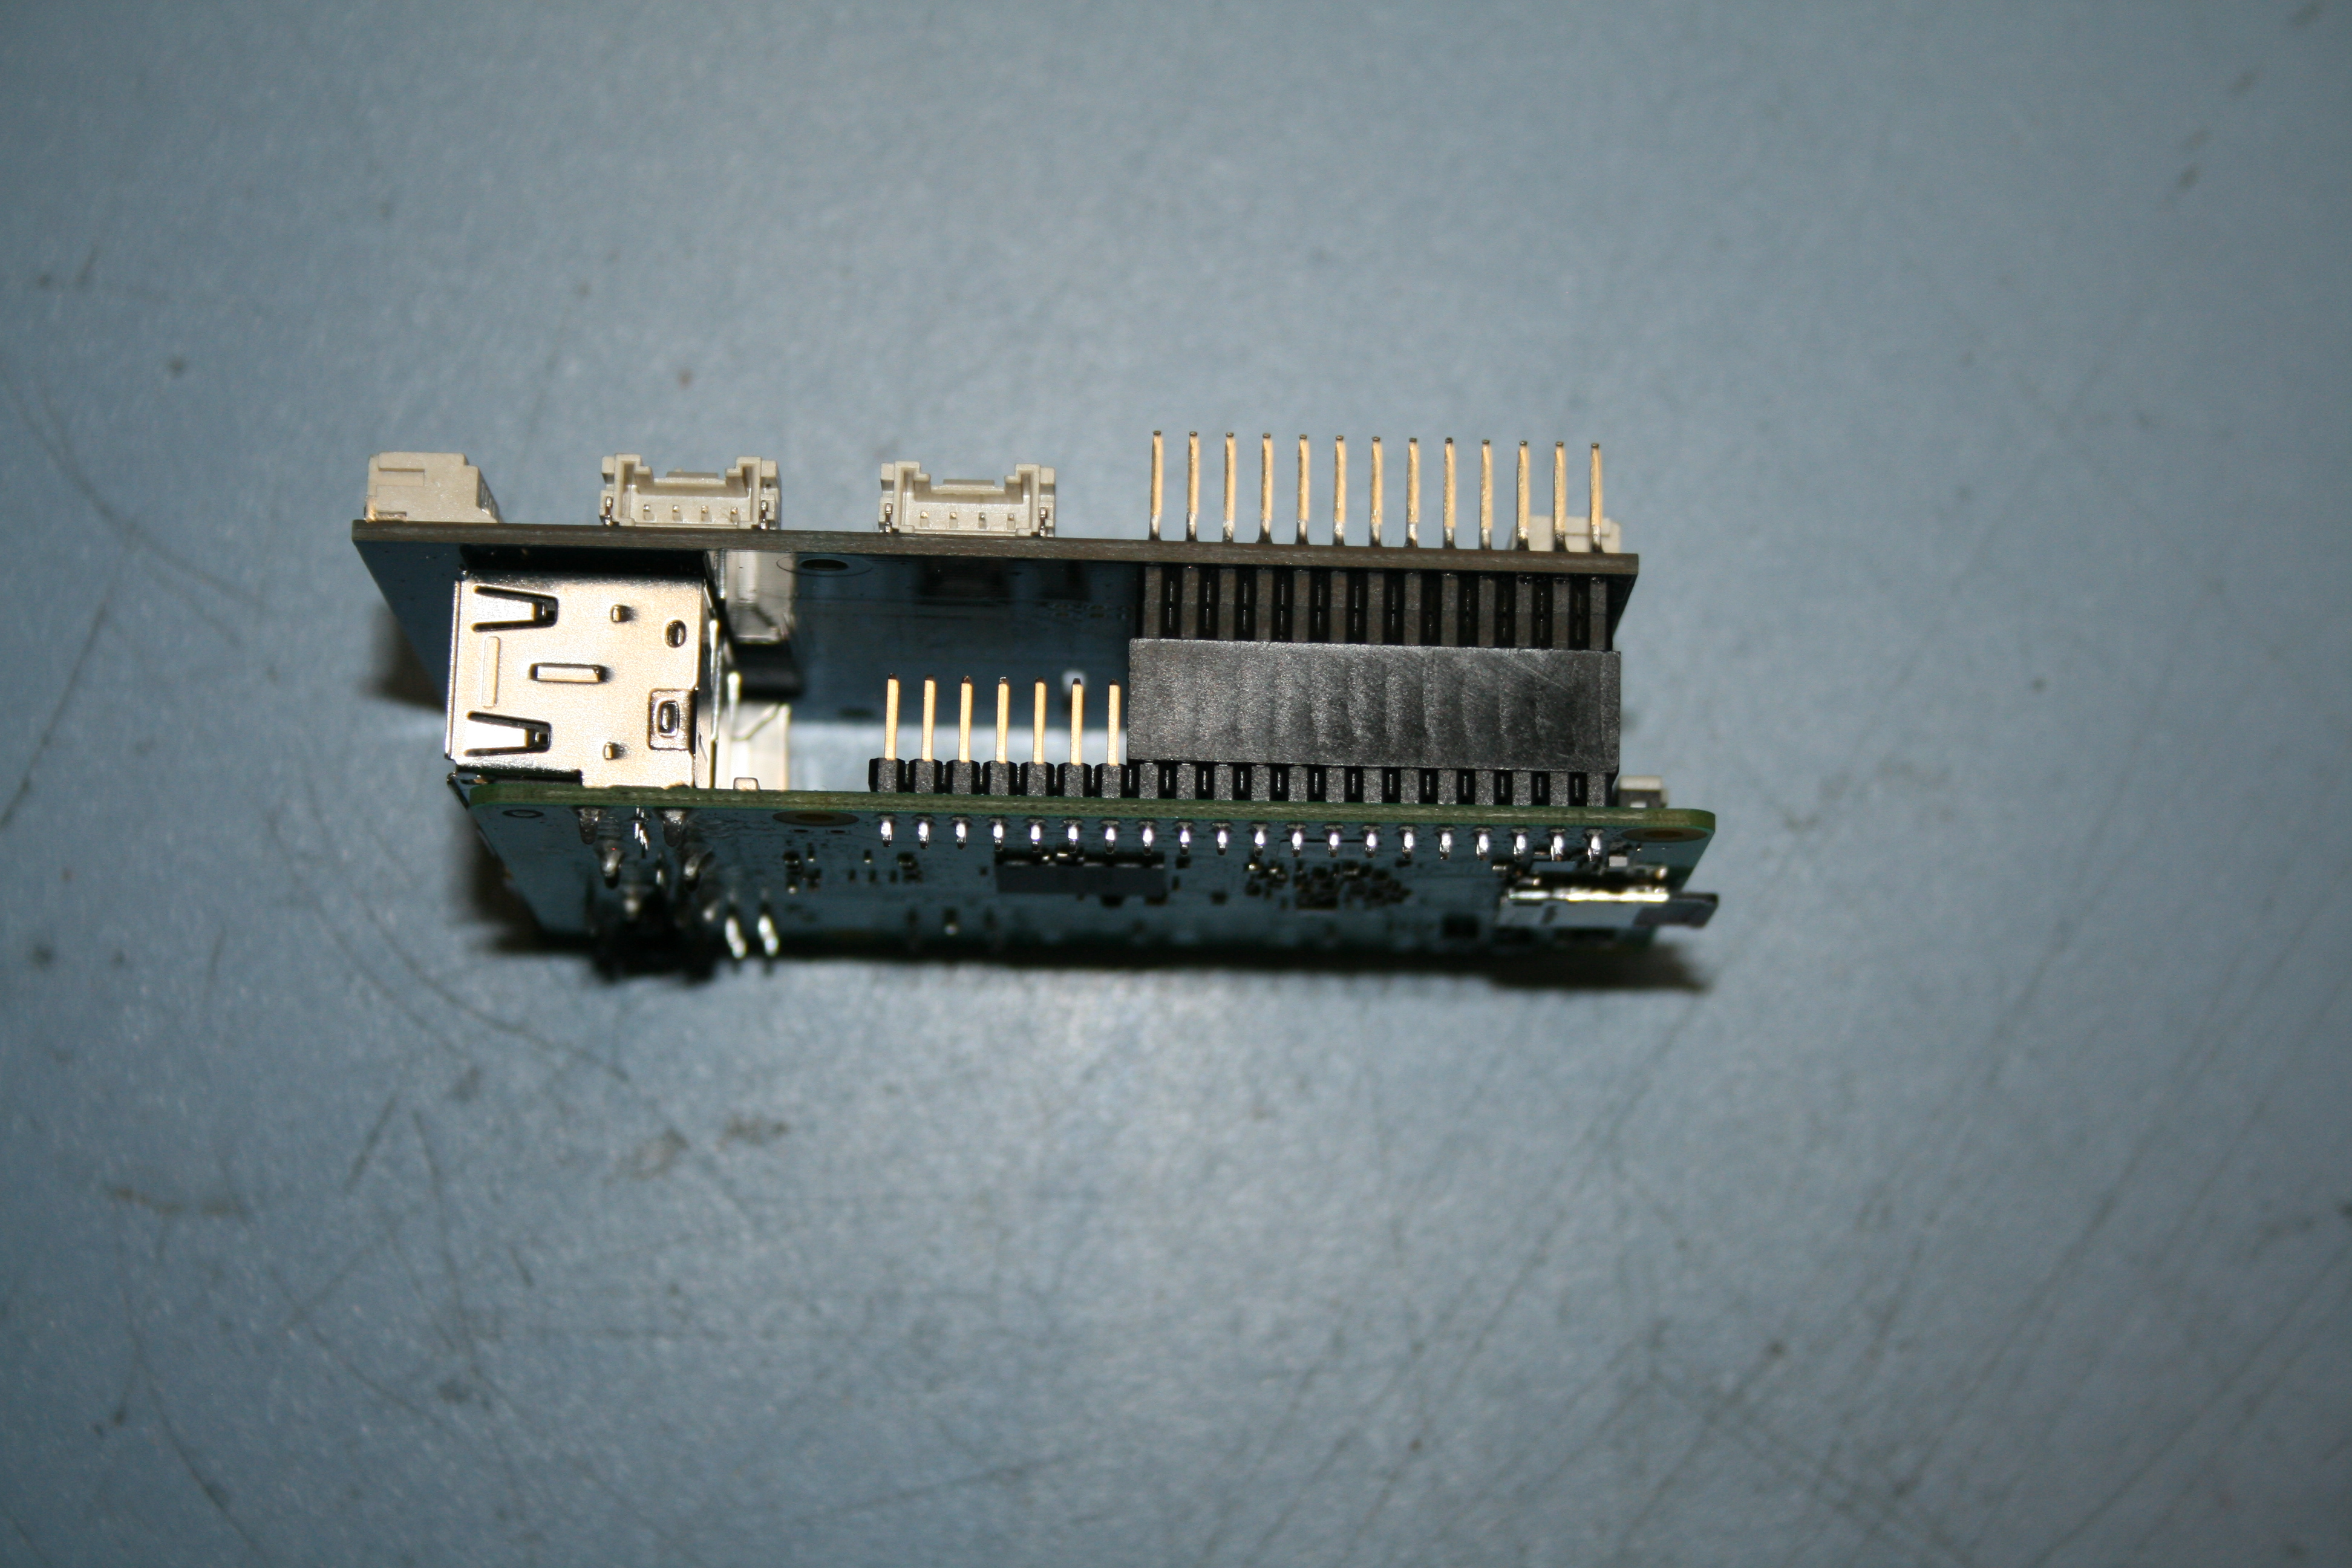
\includegraphics[width=.6\paperwidth]{images/branchement.jpg}}
	\end{center}
		\caption{ \textit{La RaspberryPi avec le Shield branché dessus}}
	\end{figure}\\
	
		\item Brancher à nouveau la \textit{RaspberryPi} au secteur. Vous devriez avoir une LED verte qui s'allume sur votre \textit{Shield}
		\item vous allez tester s'il a bien été reconnue, pour cela, connecter vous en "ssh" sur votre \textit{RaspberryPi} (vous devriez savoir le faire maintenant !)
		\item lancer la commande :
		\begin{lstlisting}[style=MyBashStyle]
	sudo i2cdetect -y 1
		\end{lstlisting}\\
	
vous devriez obtenir ce résultat, avec le 04 en première ligne.\\

\begin{figure}[H]
\begin{center}
	\makebox[\textwidth]{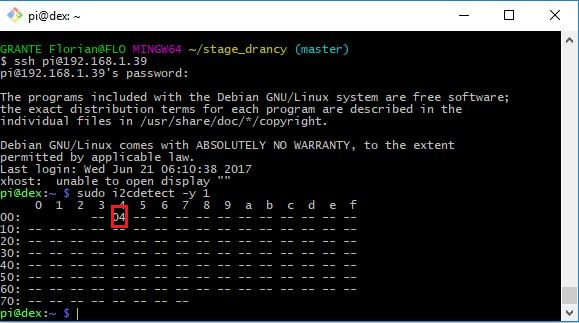
\includegraphics[width=.6\paperwidth]{images/i2cdetect.jpg}}
\end{center}
	\caption{ \textit{Test de détection du Shield}}
\end{figure}\\

\end{enumerate}\\

Voilà, la première mise en route de la \textit{RaspberryPi} est terminé. Maintenant il faut s'occuper du code pour la station final.

\newpage
\section{Installation, configuration et test du code de la station avec ses capteurs.}\\

\subsection{Installation des capteurs.}\\

Votre \textit{RaspberryPi} est configurée, ainsi que son \textit{Shield}. Il faut installer les différents capteurs. Regardons de plus près les différents connecteurs.\\

	\begin{figure}[H]
	\begin{center}
		\makebox[\textwidth]{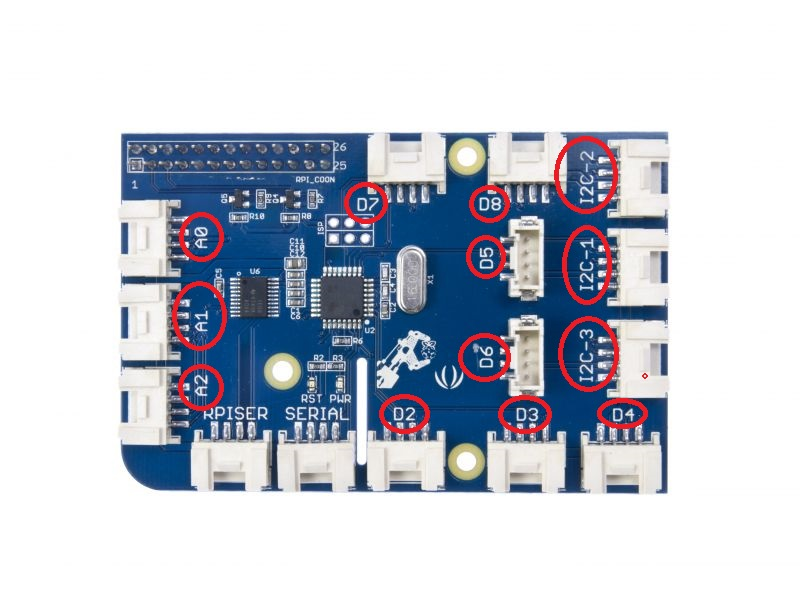
\includegraphics[width=.6\paperwidth]{images/grovepi_connecteur.jpg}}
	\end{center}
		\caption{ \textit{vu de dessus du shield}}
	\end{figure}\\
	
Comme vous pouvez le voir, il y a écrit un numéro d'identification du connecteur sur le \textit{Shield}. Vous allez donc brancher sur des ports particulier en adéquation avec le code qui sera téléchargé ultérieurement.\\

Procéder aux branchement branchements suivants :
\begin{enumerate}
	\item Le capteur de température et d'humidité (DHT11) sur le port D7.
	\item Le capteur de luminosité sur le port A1.
	\item L'encodeur rotatif sur le port A2.
	\item L'écran LCD sur un des ports I2C.
\end{enumerate}
Vous devriez alors obtenir un résultat similaire à celui là :
	\begin{figure}[H]
	\begin{center}
		\makebox[\textwidth]{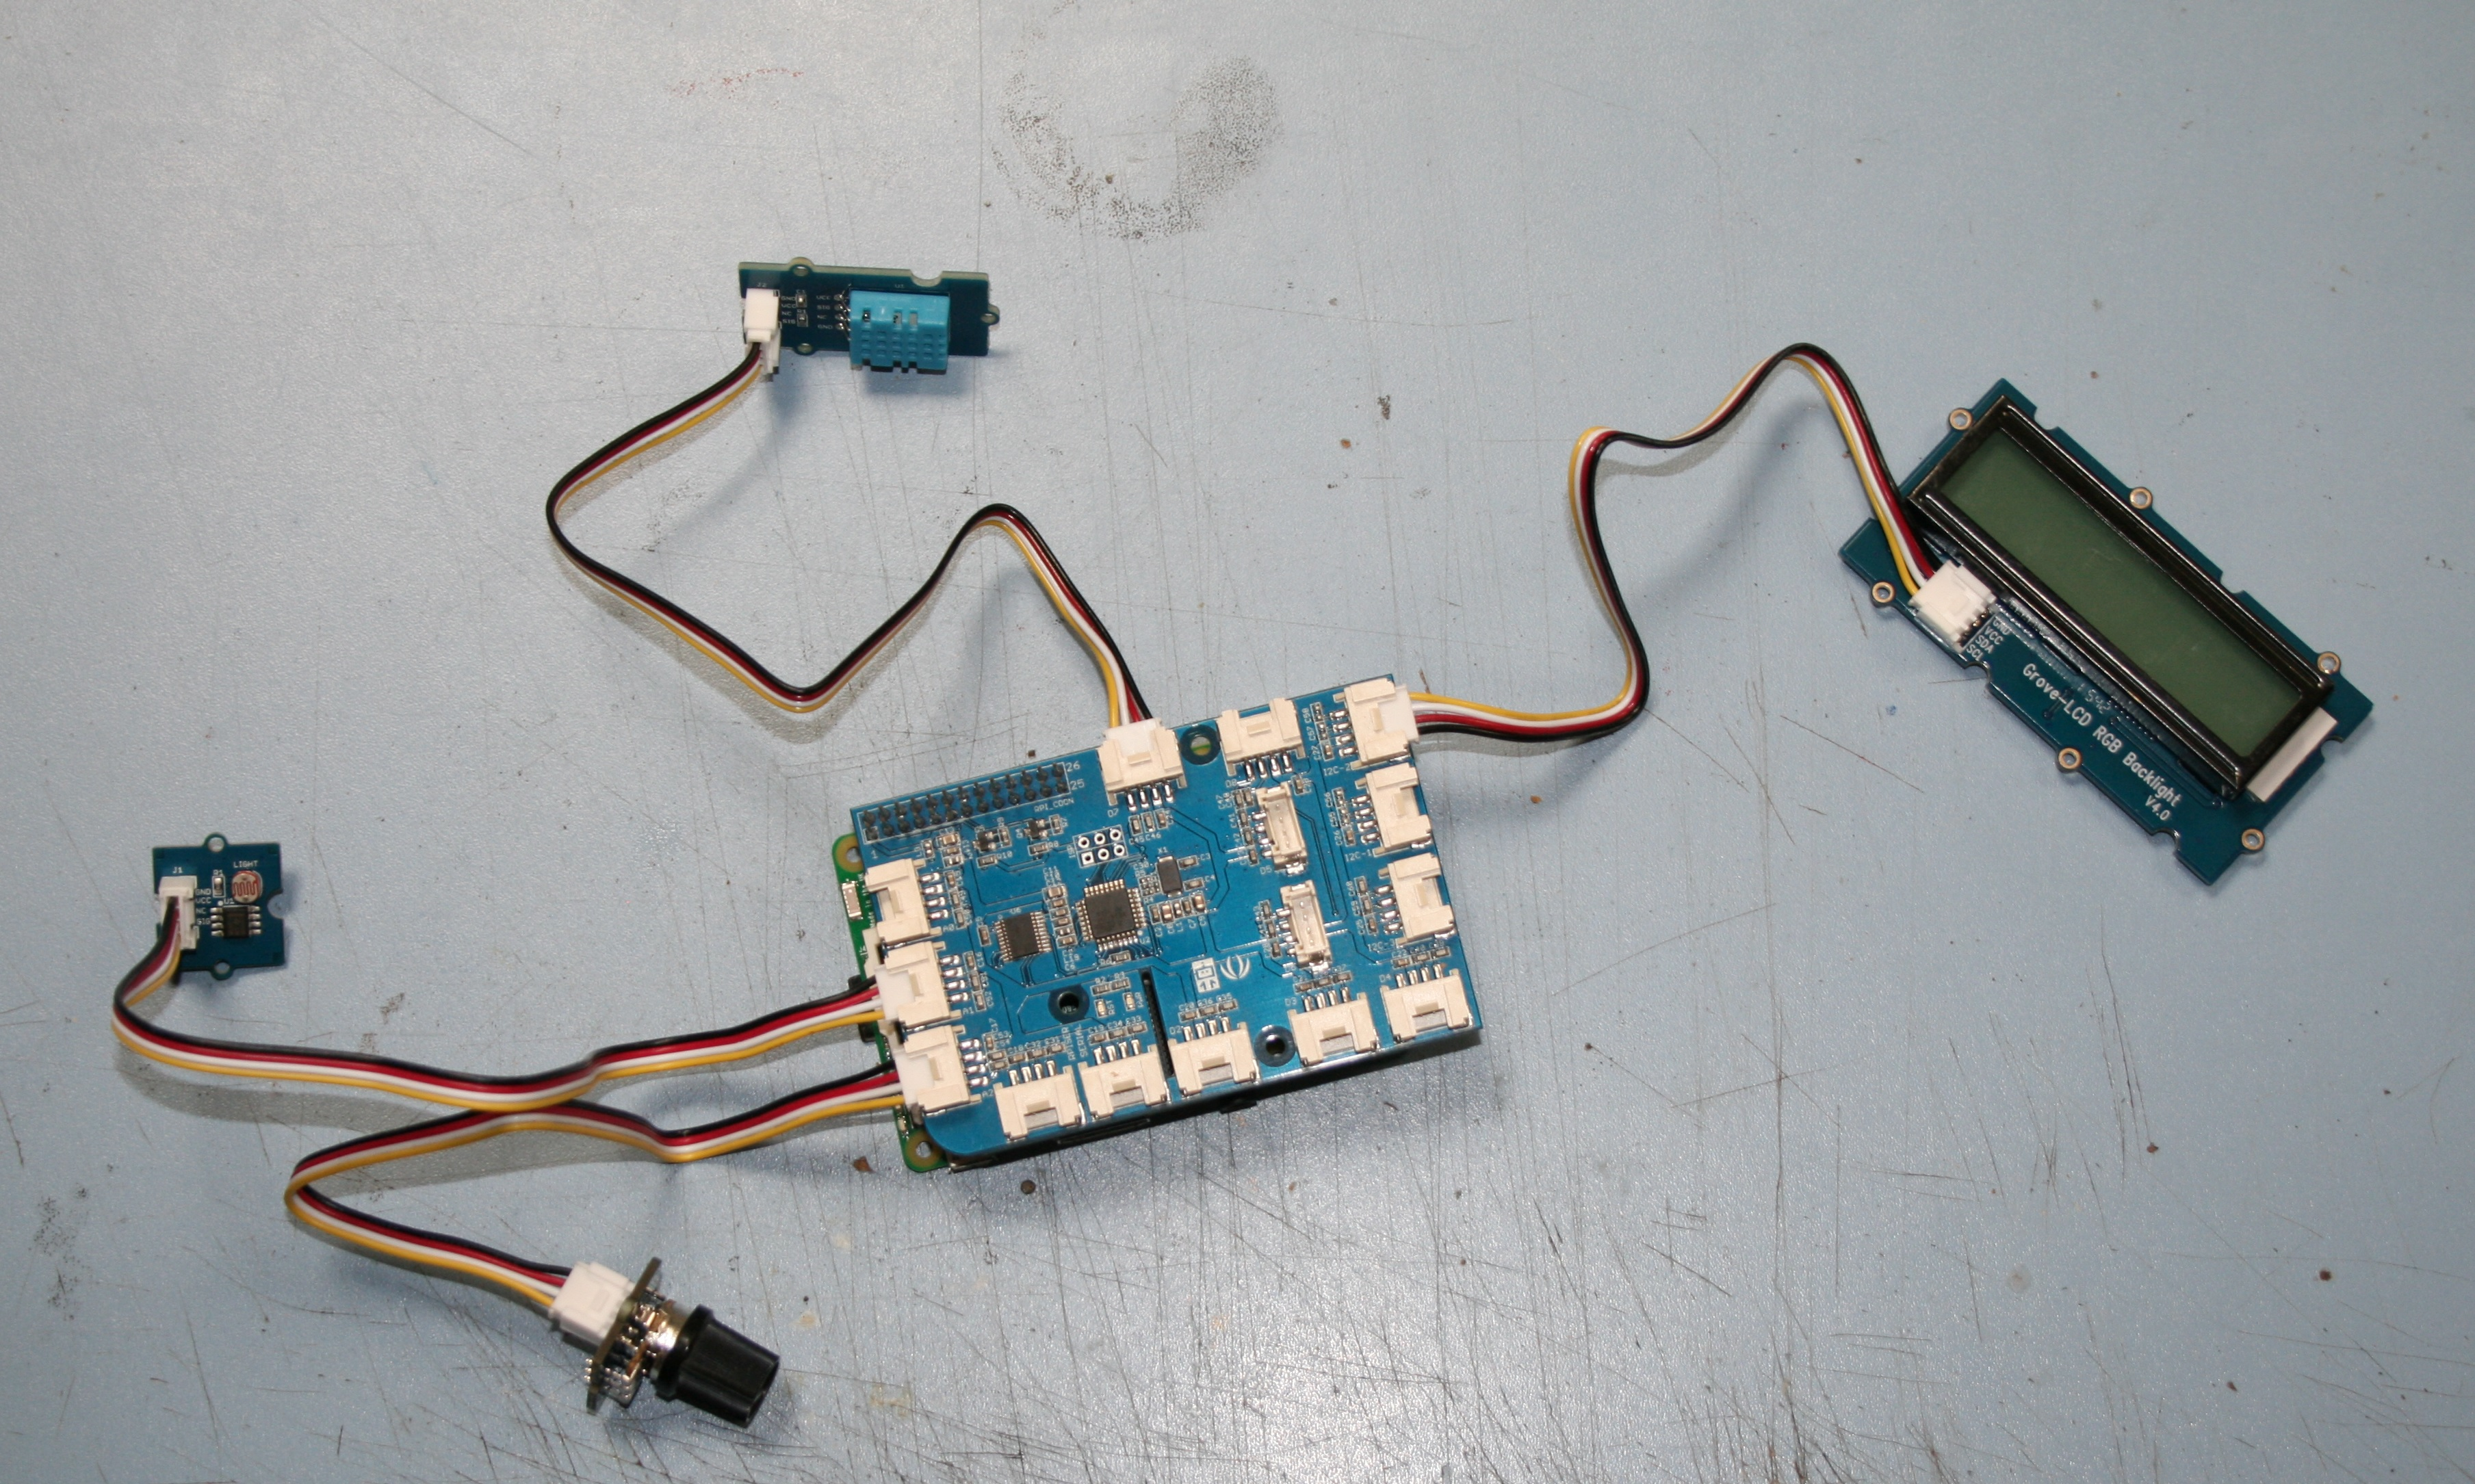
\includegraphics[width=.35\paperwidth]{images/branchement_final.jpg}}
	\end{center}
		\caption{ \textit{Branchement des compostant sur le shield}}
	\end{figure}\\

\subsection{Configuration de la \textit{RaspberryPi}.}\\

Vous allez maintenant télécharger le code pour activer le station. Pour cela, brancher votre \textit{RaspberryPi} au secteur et au réseau si jamais vous aviez enlevé le câble ethernet. Connectez vous en \textit{ssh} via \textit{git bash} et exécutez les deux commandes :\\
		\begin{lstlisting}[style=MyBashStyle]
	cd
	git clone https://github.com/Kymaro/DrancIoT
		\end{lstlisting}\\
%mettre la commande git clone du repo final

\\
Cette commande va télécharger le code nécessaire au fonctionnement de la station. Vous modifierez ce code dans le troisième chapitre pour envoyer les données sur le \textit{Cloud}.
\\

Tapez la commande :\\

\begin{lstlisting}[style=MyBashStyle]
	ls | grep DrancIoT
\end{lstlisting}\\

\begin{figure}[H]
\begin{center}
	\makebox[\textwidth]{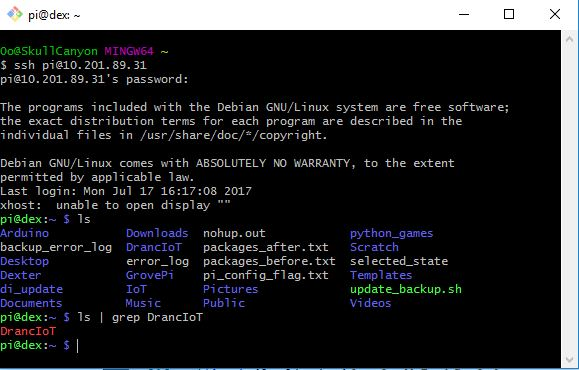
\includegraphics[width=.6\paperwidth]{images/lsgrep.jpg}}
\end{center}
	\caption{ \textit{Résultat de la commande ls avec grep}}
\end{figure}\\ 

Si vous avez bien ce résultat, cela signifie que le code à bien été téléchargé et qu'il est présent dans le dossier \textit{stage_drancy}. Si cela n'est pas le cas, réessayer la commande précédente.\\

Puis il faut faire en sorte que le script soit lancé au démarrage de la \textit{RaspberryPi}. Pour cela, il faut modifier un ficher qui gère les commandes système qui sont lancé lorsque l'OS démarre.\\

Exécuter la commande : \\

\begin{lstlisting}[style=MyBashStyle]
	sudo nano /etc/rc.local
\end{lstlisting}\\

Un fichier va alors s'ouvrir dans votre terminal, vous ne pouvez pas utiliser la souris dans cet éditeur de texte. Descendez alors avec les flèches directionnelles jusqu'à l'avant dernière ligne, la dernière ligne étant normalement \textit{exit 0}. Allez à la fin de la ligne et appuyez alors sur \textit{Entrée} pour ajouter une nouvelle ligne. 
\\
Tapez alors sur cette nouvelle ligne :\\

\begin{lstlisting}[style=MyBashStyle]
	sudo python /home/pi/DrancIoT/code/station.py &
\end{lstlisting}\\

L' esperluette permet d'exécuter le script en tâche de fond, il est important de ne pas l'oublier sinon votre \textit{RaspberryPi} ne sera pas capable de faire autre chose que de lancer votre script.

Pour quitter et enregistrer, taper sur la combinaison de touche une à une :\\

\begin{lstlisting}[style=MyBashStyle]
	Ctrl + X
	Y
	Entree
\end{lstlisting}\\

Vous êtes désormais prêt à tester la station.

\subsection{Test de la station}\\

Vous allez tout d'abord essayer la station en lançant le script manuellement pour vérifier que cela fonctionne, puis nous redémarrerons la \textit{RaspberryPi} pour voir si la modification de l'étape précédente est fonctionnelle.\\

Tapez la commande suivante pour lancer le script python.\\

NOTE : Lorsque vous indiquez le chemin d'un fichier en \textit{Bash}, vous avez votre meilleur ami qui est là pour vous aider et qui s'appelle l'auto-complétion. En effet, lorsque vous commencer à écrire le nom d'un fichier, par exemple \textit{station_cloud}, il vous suffit d'écrire \textit{sta} puis d'appuyer sur la touche \textit{Tabulation} pour voir la suite se compléter. Si cela ne se complète pas, c'est que vous avez un autre fichier / dossier qui commence par \textit{sta}, vous devez alors écrire un caractère supplémentaire pour retenter votre chance ;)\\

\begin{lstlisting}[style=MyBashStyle]
	cd
	sudo python DrancIoT/code/station.py &
\end{lstlisting}\\

Cela ne vous rappelle rien ? Il s'agit ni plus ni moins de la ligne qui a été ajoutée dans le fichier \textit{/etc/rc.local} pour démarrer automatiquement le script. (il manque /home/pi/ puisque nous sommes dans ce dossier par défaut).

Vous devriez voir l'écran LCD de la station qui s'allume avec le message "Bienvenue dans l'IoT Hub" pendant quelques seconde puis un des menus qui affiche les données des capteurs. Si cela reste sur le premier message, tourner l'encodeur rotatif pour afficher les menus.

Si vous voyez bien tous les menus avec une valeur, on y est, la station fonctionne. Vérifiez maintenant qu'elle démarre bien en même temps que la \textit{RaspberryPi}.
Mettez vous dans le scénario où elle a été coupée électriquement. 
Taper la commande :\\ %shutdown now.

\begin{lstlisting}[style=MyBashStyle]
	sudo shutdown now
\end{lstlisting}\\

Patienter quelques instants, débrancher puis rebrancher là. Vous devriez alors voir l'écran s'allumer comme pour le test précédent au bout d'un certain temps. %image.

Et voilà,vous êtes au terme de ce chapitre, vous avez désormais une station fonctionnelle localement. Je vous invite alors à suivre le chapitre trois pour configurer \textit{Microsoft Azure} d'une part puis pour modifier le code de tel sorte qu'il envoie les messages sur \textit{le Cloud Azure}.



	
	

\chapter{Configuration de \textit{Microsoft Azure}}\\

\section{Mise en place pour 1 station}\\

Vous allez abandonner notre \textit{RaspberryPi} pendant quelques instant pour se focaliser sur la création d'une instance dans le \textit{Cloud} pour que vous puissiez envoyer les données.\\

Pour réaliser cette partie, munissez vous de vos identifiant \textit{Microsoft Azure}.\\

\subsection{Explication des fonctionnalités proposées par \textit{Microsoft}}
Avant de commencer, nous allons détailler un peu plus précisément le cheminement que vont avoir nos données. Comme souvent une image vaut mieux qu'un long discours, je vous laisse observer : 
%dessin ici photoshop Hub -> Time Serie Insight

%description de l'image a faire ici

Nous allons expliciter deux méthodes différentes de gestion de \textit{Azure} pour vous montrer le champs des possible. En effet, vous pouvez utiliser le portail qui nous est proposé par \textit{Microsoft} ou bien utiliser ce qui s'appelle \textit{L'Azure CLI} pour \textit{Azure Command Line Interface}.

\subsection{Création d'un Hub d'évènements sur \textit{Azure} avec la \textit{CLI}}\\

\subsubsection{Installation de l'Interface en Ligne de Commande de \textit{Azure}}\\

Pour cette partie il n'est donc pas nécessaire de se rendre sur le portail. Mais avant toute chose, vous devez installer l'interface en ligne de commandes \textit{d'Azure}.\\

\begin{enumerate}
	\item Installer \href{https://nodejs.org/download/release/latest/}{\textit{Node.js}} en choisissant l'extension \textit{.msi} pour x64 ou x32 selon si votre système est en 64bit ou 32bit.
	\item Lancer un terminal \textit{git bash}.
	\item Tapez les deux commandes suivantes pour vérifier que \textit{Node.js}  et \textit{NPM} (Node Package Manager) a bien été installé. \textit{NPM} est l'utilitaire qui va nous permettre d'installer \textit{Azure}
	\begin{lstlisting}[style=MyBashStyle]
	node -v
	npm -v
	\end{lstlisting}\\
	Vous devriez avoir ce résultat : %photo ici
	\item Ensuite entrer la commande :
	\begin{lstlisting}[style=MyBashStyle]
	npm install -g azure-cli
	\end{lstlisting}\\
\end{enumerate}\\
Et voilà, Azure est installé, vous devriez pouvoir le lancer en tapant \textit{azure} dans votre terminal \textit{git bash}. Voici ce que vous devriez obtenir : %photo ici

\subsubsection{Création d'un groupe de ressources et d'un Hub d'évènement}\\

Maintenant, il va falloir créer nos instance qui vont récupérer les valeurs envoyée par notre station.

\begin{enumerate}
	\item Connecter vous avec votre compte \textit{Azure} :
	\begin{lstlisting}[style=MyBashStyle]
	azure login
	\end{lstlisting}\\
	Aller alors sur la page : \href{https://aka.ms/devicelog}{https://aka.ms/devicelog} pour entrer le code qui vous sera spécifié sur votre terminal. Entrer ensuite vos identifiants. Vous devriez alors être connecté. %photo ici
	\item Taper la commande :
	\begin{lstlisting}[style=MyBashStyle]
	azure group list
	\end{lstlisting}\\
Vous verrez alors la liste des groupes de ressources déjà existant. Vous allez alors créer un groupe de ressources par la commande : 
	\textbf{NOTE : POUR LE DOSSIER, LE GROUPE A POUR NOM \textit{IoT}. VOUS POUVEZ RENSEIGNER LE NOM QUE VOUS SOUHAITEZ}\\
	\begin{lstlisting}[style=MyBashStyle]
	azure group create IoT westeurope
	\end{lstlisting}\\
westeurope détermine le serveur où le groupe sera créé. %photo ici
\\
Si vous refaites la commande de l'étape N°2, vous devriez voir apparaitre votre nouveau groupe fraichement créé sur la liste.
	\item Maintenant, vous allez devoir télécharger le code de la station, comme vous l'avez fait pour la \textit{RaspberryPi} dans le chapitre 2. En effet, il y a un fichier qui sert de patron pour les paramètres à appliquer pour la commande qui suivra. Ainsi, entrer les commandes : 
	\begin{lstlisting}[style=MyBashStyle]
	cd
	git clone https://github.com/Kymaro/DrancIoT
	\end{lstlisting}\\
	\item Maintenant, vous pouvez faire la commande :
	\begin{lstlisting}[style=MyBashStyle]
azure group deployment create -g IoT -n deployment1 -f ~/DrancIoT/IoT.json
	\end{lstlisting}\\

Vous allez être inviter à entrer différentes informations. Les informations que vous allez rentrer seront indispensable car devront être ajouté au code de la station pour pouvoir envoyer les données. Les valeurs sont des chaines de caractère, celle mise en photo sont arbitraires pour le dossier, veuillez entrer une valeur différente.
	\begin{enumerate}
	\label{CLI}
		\item namespaceName : Il est conseillé de rajouter NS à la fin pour vous y retrouver ensuite. %photo ici
		\item eventHubName : Il s'agit de l'instance à proprement parlé qui va recevoir les données. vous pouvez par exemple entrer une valeur du type "Station".
		\item consumerGroupName : Pour celle valeur, je vous conseille d'entrer la même que pour namespaceName mais de remplacer NS par GN.
	\end{enumerate}\\ 
Le déploiement peut prendre un peu de temps. Si cela ne fonctionne pas, retenter en entrant des nom différents.
Une fois le déploiement terminé. Plusieurs valeurs sont à noté et sauvegarder précieusement.

\textbf{Notez d'une part la valeur des trois champs que vous avez indiquer !.
De plus, il vous faut noter la valeur de \textit{SharedAccessKeyName} et \textit{SharedAccessKey}}

\end{enumerate}

Nous en avons terminé avec la création de l'instance qui va récupérer les données envoyé par la station. Il faut maintenant vous occuper de l'instance qui va traiter les données reçu.

\subsection{Création d'un portail \textit{Time Series Insights}}

\textit{Microsoft} à pensé à nous puisque il a crée un module qui s'occupe seul de traiter les données d'une source pour ensuite créer des courbes et ainsi voir le suivi dans le temps. Sans cela, le processus aurait été nettement plus long puisqu'il aurait fallut d'une part stocké ces valeurs pour ensuite les traiter et devoir créer une interface qui puisse afficher les valeurs.

Vous allez pour cette partie nous rendre sur le \href{https://portal.azure.com}{\textit{Portail Azure}}. Nous allons dans un premier temps jeter un coup d'oeil sur le groupe que vous avez créé dans la partie d'avant. %photo ici 
\\

Cliquer à gauche sur \textit{Groupes de ressources}. Vous devriez voir apparaitre un Hub D'évènement qui porte le nom de votre \textit{namespaceName} de la partie précédente. Maintenant si vous cliquez sur ce Hub d'évènement, en bas de la vue d'ensemble devrait apparaitre un Hub d'évènement dont le nom est celui que vous avez entré pour le champs eventHubName précédemment. Une fois n'est pas coutume, continuons notre jeux des poupées russes et cliquer dessus. Une fois encore, vous devriez voir apparaitre en bas deux groupe de consommateur. Le premier, \textit{Default} est.... celui utilisé par défaut si jamais vous ne voulez pas créer de groupe de consommateur. Mais c'est toujours mieux d'en avoir un dont on connait le nom par soucis de visibilité. Le second est celui que vous avez créé tout à l'heure.\\

Maintenant que vous êtes rassuré sur les lignes de commande de la partie précédente nous allons pouvoir créer notre instance de traitement des données.\\
\begin{enumerate}
	\item Cliquer sur le \textit{+} en haut à gauche de votre portail.
	\item Dans la barre de recherche du menu qui vient de s'ouvrir, entrer \textit{"Time Series"}
	\item Choisissez alors \textit{"Time Series Insights (aperçu)}
	
\begin{figure}[H]
\begin{center}
	\makebox[\textwidth]{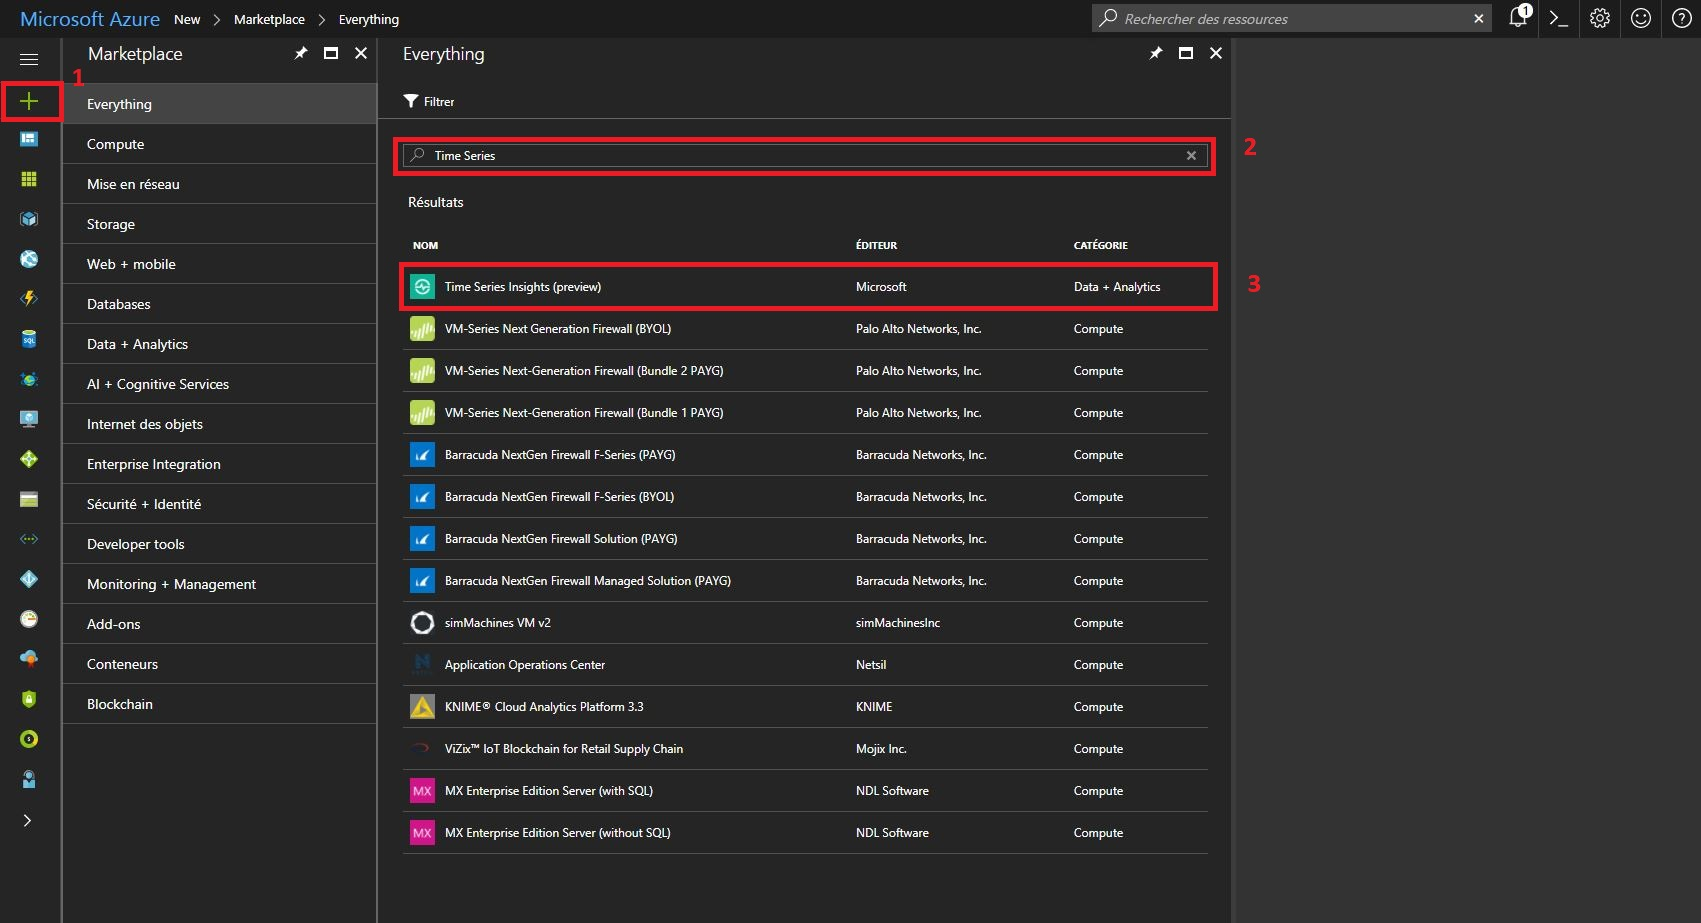
\includegraphics[width=.7\paperwidth]{images/azure_portal_1.jpg}}
\end{center}
	\caption{ \textit{Menu de recherche de ressources sur Azure}}
\end{figure}\\

	\item Cliquer alors sur \textit{Créer}.\\
Vous arrivez alors sur la fenêtre  suivante :\\

\begin{figure}[H]
\begin{center}
	\makebox[\textwidth]{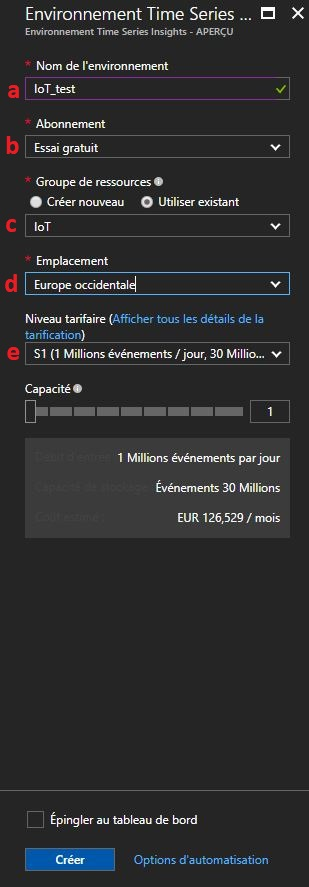
\includegraphics[width=.4\paperwidth]{images/azure_portal_2.jpg}}
\end{center}
	\caption{ \textit{Menu de recherche de ressources sur Azure}}
\end{figure}\\

\begin{enumerate}

	\item Il s'agit du nom que vous voulez donner à votre Portail. Ce nom apparaitra sur le Portail, donc préférez un nom qui vous indique les données qui vont y être envoyer.
	
	\item Choisissez votre abonnement \textit{azure}.
	
	\item Choisissez le groupe de ressources que nous avons créée tout à l'heure. Pour le dossier, il s'agissait du groupe \textit{"IoT"}.
	\item Sélectionner \textit{"Europe Occidentale"}. C'est le serveur sur lequel va être implanté le portail.
	
	\item Pour ce choix, cela dépendra de votre besoin. Sachez que ce choix détermine le tarif du portail. Pour information, la station envoie ses données environ toute les deux minutes. Il n'était pas possible de mettre un délai plus long auquel cas il y aurait des problème de déconnexion de la station. Partez du principe qu'une station envoie 1000 évènements par jour, cela vous donne une indication quant aux nombre de stations que vous pouvez implémenter sur le portail.
	\item Cliquer alors sur \textit{Créer}.
	
\end{enumerate} \\
\end{enumerate}

Voilà, votre portail est en cours de déploiement, nous allons maintenant devoir faire en sorte que cette instance écoute les valeurs que l'on envoie sur le Hub d'évènement.

\subsection{Ajout d'une source d'évènements dans le portail \textit{Time Series Insights}}

Maintenant que vous avez créer votre instance \textit{Time Series Insights}, cliquer dessus pour voir sa page principale affichée :\\

\begin{figure}[H]
\begin{center}
	\makebox[\textwidth]{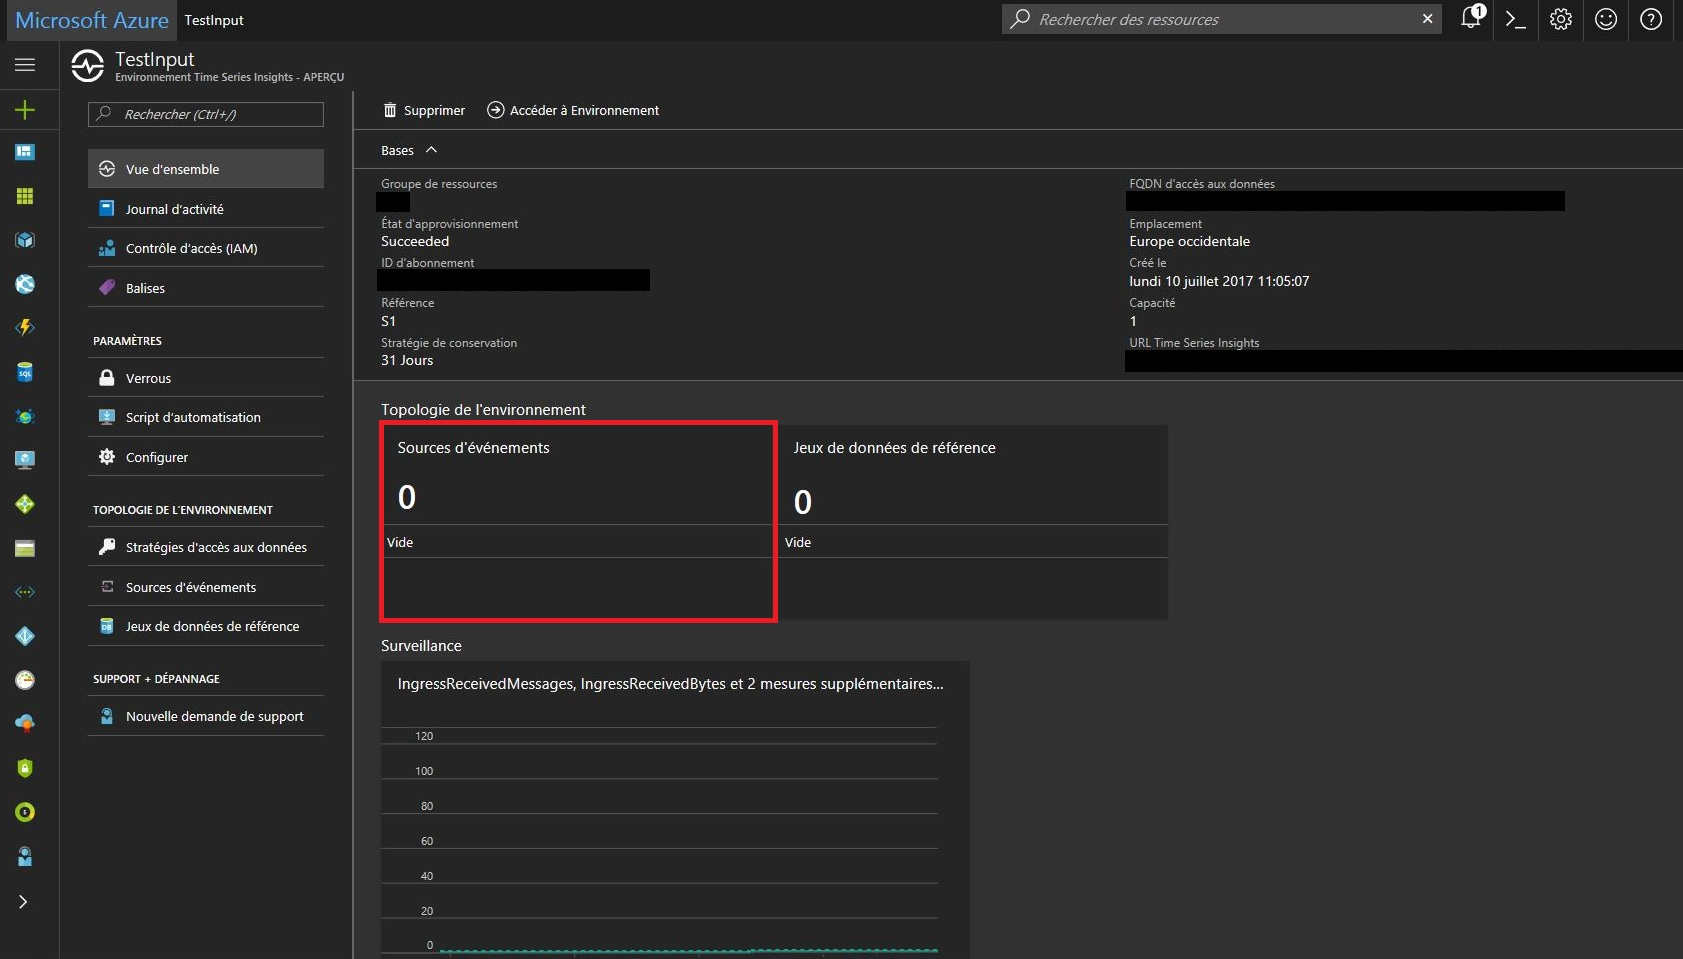
\includegraphics[width=.7\paperwidth]{images/azure_portal_3.jpg}}
\end{center}
	\caption{ \textit{Menu principal du \textit{Time Series Insights}}}
\end{figure}\\

\begin{enumerate}
	\item Cliquer sur la zone \textit{Sources d'évènements} puis sur \textit{Ajouter} en haut dans la fenêtre qui s'ouvrira.
	\item vous devriez alors voir apparaitre cette fenêtre : 
	\begin{figure}[H]
\begin{center}
	\makebox[\textwidth]{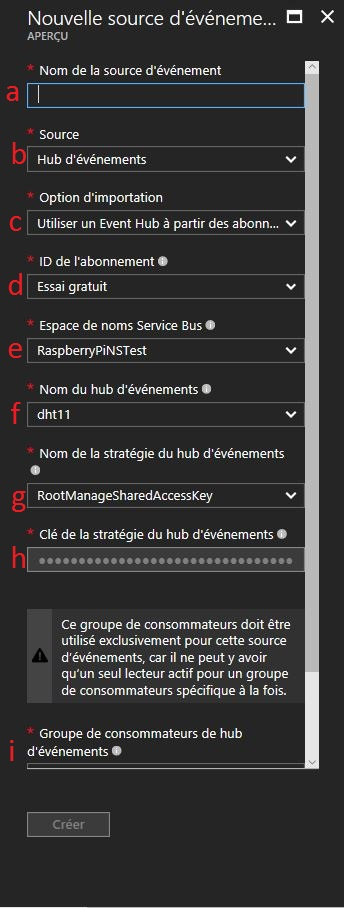
\includegraphics[width=.4\paperwidth]{images/azure_portal_4.jpg}}
\end{center}
	\caption{ \textit{Ajout d'une source d'évènements}}
\end{figure}\\
	\begin{enumerate}
	\item C'est le nom que vous voulez donner à votre source. Le choix est arbitraire.
	\item Choisir \textit{Hub d'évènements}.
	\item Choisi \textit{Utiliser un Event Hub à partir des abonn..}
	\item Ici, le champs dépend de votre abonnement.
	\item Pour les étapes qui vont suivre, il sera nécessaire de reprendre les champs indiqué lors de la section~\ref{CLI} page~\pageref{CLI}. Pour le premier, entrer le \textit{namespaceName}.
	\item Ici doit être indiqué \textit{l'evenHubName}.
	\item Le choix \textit{RootManageSharedAccessKey} devrait être proposé. Il s'agit probablement de votre \textit{SharedAccessKeyName}. Sinon, renseigner votre \textit{SharedAccessKeyName}
	\item Renseigner votre \textit{SharedAccessKey}
	\item Ici doit être entré votre \textit{consumerGroupName}.
	\item laisser ce dernier champs vide et cliquer sur \textit{Créer}.
	\end{enumerate}
\end{enumerate}\\

Vous avez donc ajouté le hub d'évènement comme source pour l'instance de \textit{Time Series Insights}. Il reste alors à éditer le code de la station pour indiquer le hub sur lequel envoyer les données.


\subsection{Configuration logiciel de la station pour \textit{Azure}}

Avant de vous montrer les modifications à réaliser dans le code, quelques informations concernant celui ci. Le code est écrit dans le langage \href{https://www.python.org/}{Python}. En plus d'avoir le mérite d'être considéré comme un des langages les plus haut niveau (ie. proche du langage de l'Homme et donc intuitif), il est particulièrement adapté pour l'utilisation de script automatisé comme vous allez le faire pour la station.\\

\textbf{ATTENTION : Avant de vous faire découvrir le code et de vous expliquer les lignes à modifier pour pouvoir envoyer vos données, une petite explication sur l'architecture d'un code Python. Il est impératif de respecter les indentations (espacement) du code. Si jamais vous rajouter ne serait-ce qu'un espace sur une ligne, cela peut avoir comme effet de faire planter l'intégralité de la station. Si cela ce produit, pour simplifier le problème, reportez vous à l'annexe N°1.}\\

Il reste cependant une étape avant de modifier le code. En effet, il est nécessaire d'installer la bibliothèque azure sur la \textit{RaspberryPi}. Pour cela, connectez vous en ssh dessus puis entrer la commande :\\

\begin{lstlisting}[style=MyBashStyle]
	sudo pip install azure-servicebus
\end{lstlisting}\\

Nous pouvons désormais regarder le code :\\ 
\newpage
\pythonexternal{../../DrancIoT/code/station.py}\\

Maintenant que vous avez le code à disposition avec les lignes, vous allez pouvoir réaliser les changements de manière un peu plus lisible. Pour éditer le fichier, effectuer la commande :

\begin{lstlisting}[style=MyBashStyle]
	sudo nano /home/pi/DrancIoT/code/station.py
\end{lstlisting}\\

Modifier alors les lignes suivantes : 
\begin{enumerate} %numero de ligne a changer dans la version final
	\item Ligne 6 & 7 : Retirer le dièze pour importer les bibliothèques azure que vous venez d'installer.
	\item Ligne 29 : Il s'agit de l'identifiant qui caractérisera votre station dans le portail \textit{Azure}. indiquer donc une chaine de caractère qui vous permettra ensuite d'identifier qu'elle station elle représente sur \textit{Azure}. Cet identifiant permettra de classer les stations.
	\item Ligne 57 à 67 : Supprimer, lorsqu'il y en a un, le dièze.
	\item Ligne 60 : Indiquer entre les ' votre \textit{namespaceName} créer avec la \textit{CLI}.
	\item Ligne 61 : Indiquer toujours entre les ' votre \textit{SharedAccessKeyName}.
	\item Ligne 62 : de la même façon indiquer la \textit{SharedAccessKey}.
	\item Ligne 69 : Retirer le dièze.
	\item Ligne 83 : Retirer le dièze et remplacer dans les ' par votre \textit{eventHubName} créé avec le \textit{CLI}. 
\end{enumerate}

La station est maintenant prête à l'emploie. Nous allons pouvoir la tester. Pour cela faite la commande :\\

\begin{lstlisting}[style=MyBashStyle]
	sudo reboot
\end{lstlisting}\\

Rendez vous sur la page principal du \textit{Time Series Insights} puis cliquer sur \textit{Accéder à l'Environnement} en haut de cette page pour voir apparaitre le portail avec les données.

\subsection{Affichage et traitement des données sur \textit{Time Series Insights}}

Voici ce a quoi vous devez vous attendre sur le \textit{Time Series Insights} : \\

\begin{figure}[H]
\begin{center}
	\makebox[\textwidth]{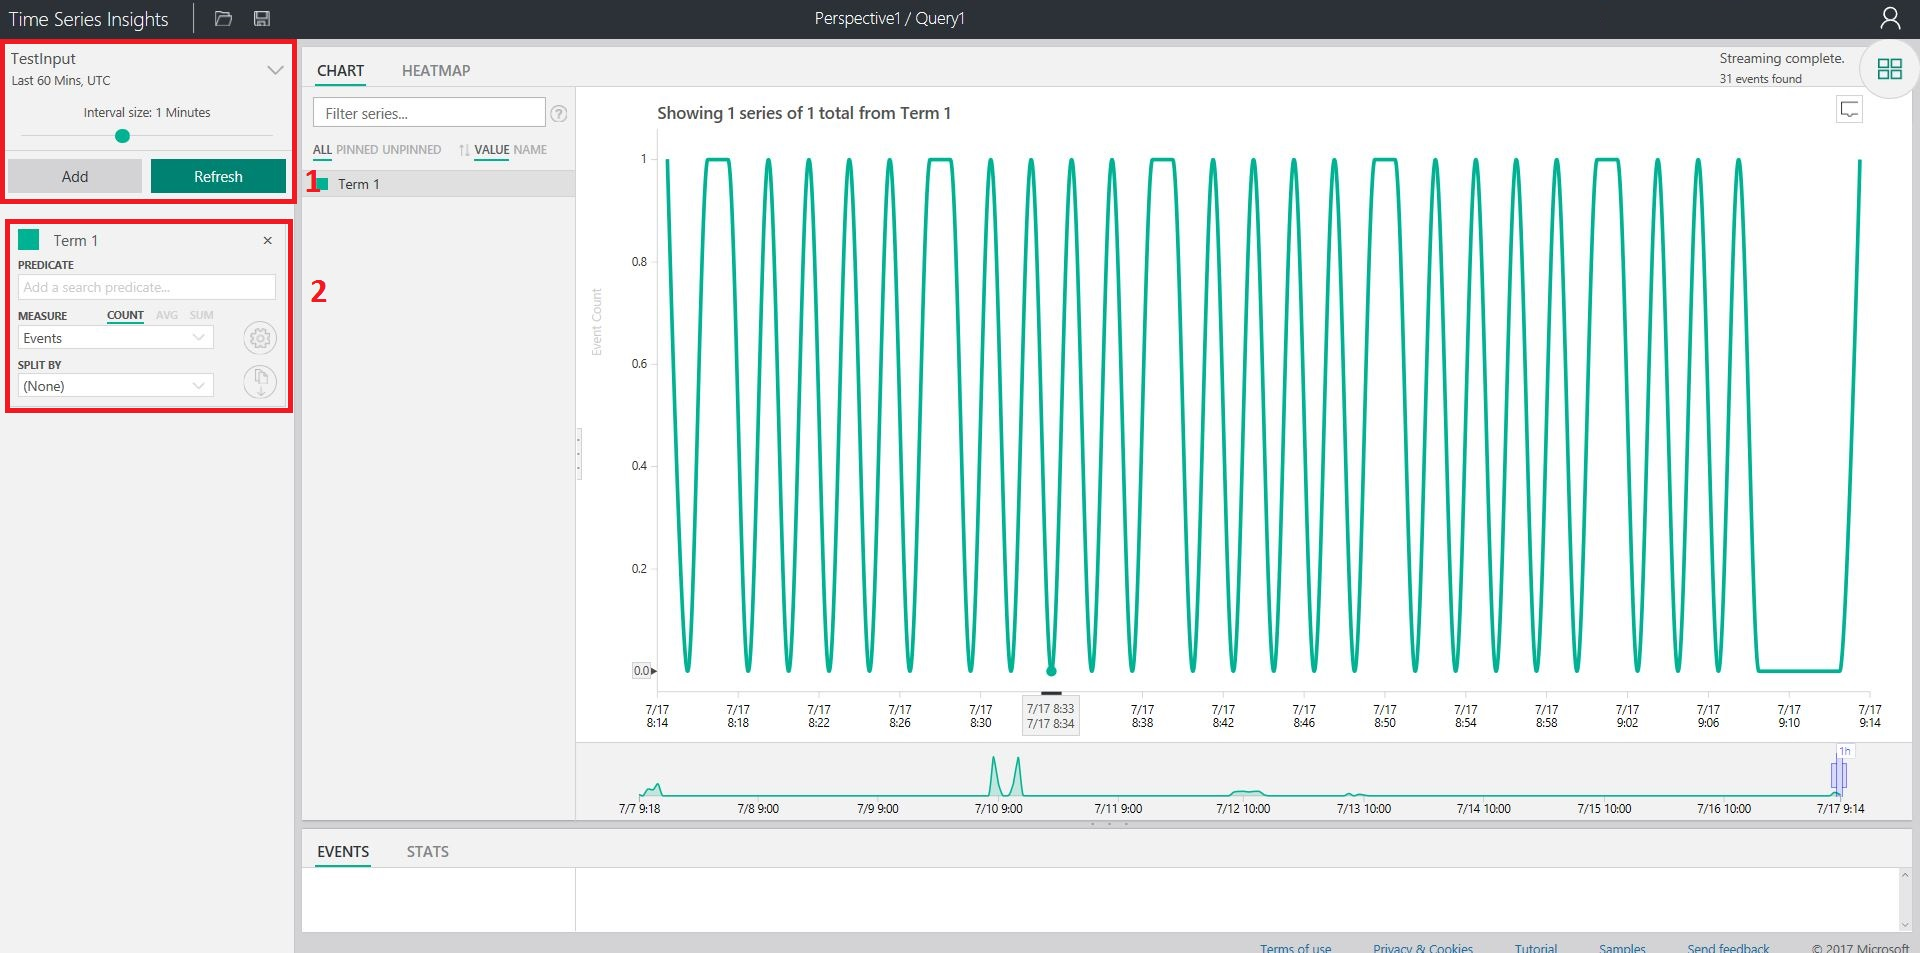
\includegraphics[width=.7\paperwidth]{images/time_1.jpg}}
\end{center}
	\caption{ \textit{Le portail \textit{Time Series Insights}}}
\end{figure}\\

Je vous ai mis en évidence 2 zones. 
\begin{enumerate}
\item La première zone vous permet de choisir une fenêtre temporelle pour regarder vos données. Si vous cliquer dessus, vous verrez apparaitre le menu suivant :\\

\begin{figure}[H]
\begin{center}
	\makebox[\textwidth]{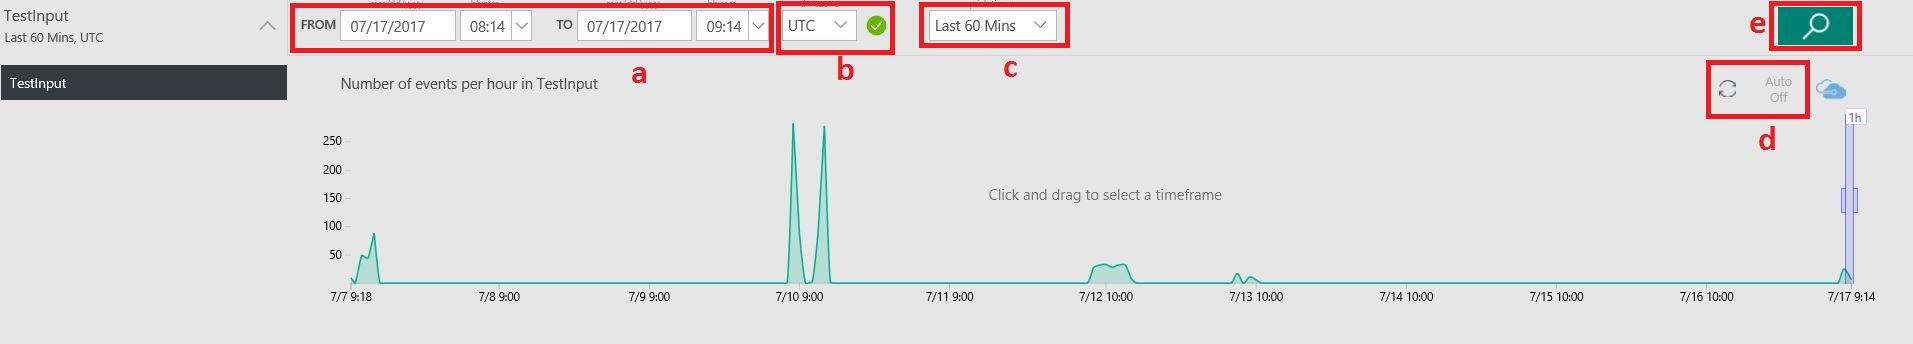
\includegraphics[width=.7\paperwidth]{images/time_2.jpg}}
\end{center}
	\caption{ \textit{Choix de la tranche horaire}}
\end{figure}\\

\begin{enumerate}
\item Vous pouvez choisir une tranche horaire personnalisé avec un point de départ et un point d'arrivé.
\item Attention à ce menu déroulant. Veillez à bien choisir \textit{Local}.
\item Vous pouvez choisir des fenêtre déjà créée qui prennent les dernière valeur sur un temps voulue.
\item les flèches vous permette de mettre à jour les valeurs reçu. Si vous cliquer sur \textit{Auto off}, ce la passera en mode \textit{Auto On} qui est donc le rafraîchissement automatique.
\item Enfin cliquer sur la loupe pour appliquer votre sélection.
\end{enumerate}

\item La seconde zone représente la courbe que vous affichez à l'écran.
\begin{enumerate}
\item Le premier menu déroulant vous permet de choisir la donnée que vous voulez afficher. Vous aurez alors le choix entre  \textit{la Temperature},\textit{l'Humidité} ou encore \textit{La luminosité}.
\item Le second menu déroulant vous permet de choisir comment distinguer les évènements que vous recevez. Choisissez alors \textit{DevideID} pour séparer les évènements par \textit{station}. 
\end{enumerate}
\end{enumerate}

% ajouter le control d'acces des compte au portail.












	
	





\chapter*{Conclusion}

\addcontentsline{toc}{chapter}{Conclusion}

Ce dossier avait pour objectif la mise en place de stations dans le but d'installer une solution de monitoring de bâtiment. Même s'il est évident qu'il existe des dizaines de façon de le faire, celle qui vous est proposée est probablement la plus simple d'un point de vue technique dans les solutions non propriétaire car il ne fallait aucun pré-requis pour utiliser ce dossier.\\

Au-delà de son objectif principal, il vous aura, je l'espère, apporté quelques compétences en manipulation système avec le langage \textit{Bash} et une certaine initiation de l'électronique embarqué.
\newpage
\chapter*{Annexes}
\addcontentsline{toc}{chapter}{Annexes}

\section*{Annexe 1 : Remise à 0 du code}
\addcontentsline{toc}{section}{Annexe 1 : Remise à 0 du code}
\label{ANNEXE1}
Cette annexe est utile si jamais vous avez téléchargé le code au travers de la commande : 

\begin{lstlisting} [style=MyBashStyle]
	git clone https://github.com/Kymaro/DrancIoT.git
\end{lstlisting}\\

Si jamais vous avez fait des modifications du code et que vous êtes dans l'incapacité de revenir en arrière sur votre \textit{RaspberryPi}. Si vous êtes encore dans l'éditeur de fichier, fermer le terminal pour vous déconnecter de la \textit{RaspberryPi}. Connectez vous à nouveau en \textit{SSH} sur votre station et effectuer les étapes :\\

\begin{lstlisting} [style=MyBashStyle]

	cd
	cd DrancIoT/
	git reset --hard
\end{lstlisting}\\

Les fichiers devraient alors revenir à leur état initial comme si vous veniez de le télécharger. Vous pouvez alors recommencer la sous-partie~\ref{CONFIG} page~\pageref{CONFIG} \textbf{sans recommencer la commande :}\\

\begin{lstlisting}[style=MyBashStyle]
	sudo pip install azure-servicebus
\end{lstlisting}\\


\section*{Annexe 2 : Alimentation PoE de la \textit{RaspberryPi}}
\addcontentsline{toc}{section}{Annexe 2 : Alimentation PoE de la \textit{RaspberryPi}}\\

L'une des conditions du cahier des charges était que la station soit alimenté en PoE. PoE est l'anagramme de "Power over Ethernet". Comprenez en français "Alimentation électrique par câble Ethernet". Il faut savoir qu'en plus d'assurer le transfert de données, un câble réseaux peut, par cette technologie, alimenter des périphériques.\\

Le câble délivre alors une tension de 48V pour une puissance maximal d'environ 13 Watts. 

	Cela signifie que votre station sera alimenté non pas par une prise secteur classique, mais bel et bien par son câble ethernet au travers de sa prise RJ45 de la \textit{RaspberryPi}. Malheureusement cette dernière ne gère pas la technologie PoE. Elle ne peut donc pas convertir l'alimentation 48V qu'elle recevrait en alimentation 5V dont elle a besoin. C'est pour cette raison que vous allez utiliser un \textit{PoE Splitter}.
	
	\begin{figure}[H]
	\begin{center}
		\makebox[\textwidth]{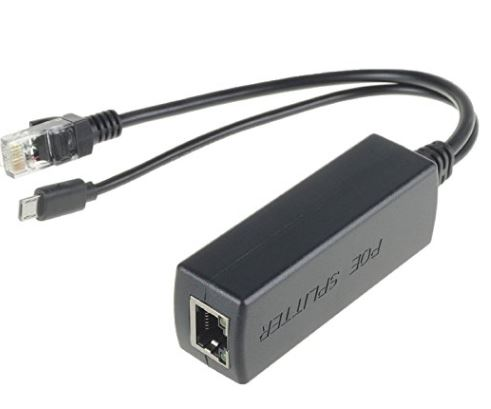
\includegraphics[width=.6\paperwidth]{images/PoE.jpg}}
	\end{center}
		\caption{ \textit{PoE Splitter}}
	\end{figure}\\
	
Ce petit adaptateur vous permettra, comme vous pouvez le voir, de séparer l'alimentation PoE et les données dans un connecteur respectivement micro USB et RJ45. De cette façon, nous pouvons alimenter notre station en \textit{PoE}.
\newpage
\nocite{*}

\end{document}